\documentclass[12pt,a4paper,]{book}
\def\ifdoblecara{} %% set to true
\def\ifprincipal{} %% set to true
\let\ifprincipal\undefined %% set to false
\def\ifcitapandoc{} %% set to true
\let\ifcitapandoc\undefined %% set to false
\usepackage{lmodern}
\usepackage{amssymb,amsmath}
\usepackage{ifxetex,ifluatex}
%\usepackage{fixltx2e} % provides \textsubscript %PLLC
\ifnum 0\ifxetex 1\fi\ifluatex 1\fi=0 % if pdftex
  \usepackage[T1]{fontenc}
  \usepackage[utf8]{inputenc}
\else % if luatex or xelatex
  \ifxetex
    \usepackage{mathspec}
  \else
    \usepackage{fontspec}
  \fi
  \defaultfontfeatures{Ligatures=TeX,Scale=MatchLowercase}
\fi
% use upquote if available, for straight quotes in verbatim environments
\IfFileExists{upquote.sty}{\usepackage{upquote}}{}
% use microtype if available
\IfFileExists{microtype.sty}{%
\usepackage{microtype}
\UseMicrotypeSet[protrusion]{basicmath} % disable protrusion for tt fonts
}{}
\usepackage[margin = 2.5cm]{geometry}
\usepackage{hyperref}
\hypersetup{unicode=true,
            pdfauthor={Nombre Completo Autor},
              pdfborder={0 0 0},
              breaklinks=true}
\urlstyle{same}  % don't use monospace font for urls
\usepackage{natbib}
\bibliographystyle{plainnat}
\usepackage[usenames,dvipsnames]{xcolor}  %new PLLC
\usepackage{color}
\usepackage{fancyvrb}
\newcommand{\VerbBar}{|}
\newcommand{\VERB}{\Verb[commandchars=\\\{\}]}
\DefineVerbatimEnvironment{Highlighting}{Verbatim}{commandchars=\\\{\}}
% Add ',fontsize=\small' for more characters per line
\usepackage{framed}
\definecolor{shadecolor}{RGB}{248,248,248}
\newenvironment{Shaded}{\begin{snugshade}}{\end{snugshade}}
\newcommand{\AlertTok}[1]{\textcolor[rgb]{0.94,0.16,0.16}{#1}}
\newcommand{\AnnotationTok}[1]{\textcolor[rgb]{0.56,0.35,0.01}{\textbf{\textit{#1}}}}
\newcommand{\AttributeTok}[1]{\textcolor[rgb]{0.77,0.63,0.00}{#1}}
\newcommand{\BaseNTok}[1]{\textcolor[rgb]{0.00,0.00,0.81}{#1}}
\newcommand{\BuiltInTok}[1]{#1}
\newcommand{\CharTok}[1]{\textcolor[rgb]{0.31,0.60,0.02}{#1}}
\newcommand{\CommentTok}[1]{\textcolor[rgb]{0.56,0.35,0.01}{\textit{#1}}}
\newcommand{\CommentVarTok}[1]{\textcolor[rgb]{0.56,0.35,0.01}{\textbf{\textit{#1}}}}
\newcommand{\ConstantTok}[1]{\textcolor[rgb]{0.00,0.00,0.00}{#1}}
\newcommand{\ControlFlowTok}[1]{\textcolor[rgb]{0.13,0.29,0.53}{\textbf{#1}}}
\newcommand{\DataTypeTok}[1]{\textcolor[rgb]{0.13,0.29,0.53}{#1}}
\newcommand{\DecValTok}[1]{\textcolor[rgb]{0.00,0.00,0.81}{#1}}
\newcommand{\DocumentationTok}[1]{\textcolor[rgb]{0.56,0.35,0.01}{\textbf{\textit{#1}}}}
\newcommand{\ErrorTok}[1]{\textcolor[rgb]{0.64,0.00,0.00}{\textbf{#1}}}
\newcommand{\ExtensionTok}[1]{#1}
\newcommand{\FloatTok}[1]{\textcolor[rgb]{0.00,0.00,0.81}{#1}}
\newcommand{\FunctionTok}[1]{\textcolor[rgb]{0.00,0.00,0.00}{#1}}
\newcommand{\ImportTok}[1]{#1}
\newcommand{\InformationTok}[1]{\textcolor[rgb]{0.56,0.35,0.01}{\textbf{\textit{#1}}}}
\newcommand{\KeywordTok}[1]{\textcolor[rgb]{0.13,0.29,0.53}{\textbf{#1}}}
\newcommand{\NormalTok}[1]{#1}
\newcommand{\OperatorTok}[1]{\textcolor[rgb]{0.81,0.36,0.00}{\textbf{#1}}}
\newcommand{\OtherTok}[1]{\textcolor[rgb]{0.56,0.35,0.01}{#1}}
\newcommand{\PreprocessorTok}[1]{\textcolor[rgb]{0.56,0.35,0.01}{\textit{#1}}}
\newcommand{\RegionMarkerTok}[1]{#1}
\newcommand{\SpecialCharTok}[1]{\textcolor[rgb]{0.00,0.00,0.00}{#1}}
\newcommand{\SpecialStringTok}[1]{\textcolor[rgb]{0.31,0.60,0.02}{#1}}
\newcommand{\StringTok}[1]{\textcolor[rgb]{0.31,0.60,0.02}{#1}}
\newcommand{\VariableTok}[1]{\textcolor[rgb]{0.00,0.00,0.00}{#1}}
\newcommand{\VerbatimStringTok}[1]{\textcolor[rgb]{0.31,0.60,0.02}{#1}}
\newcommand{\WarningTok}[1]{\textcolor[rgb]{0.56,0.35,0.01}{\textbf{\textit{#1}}}}
\IfFileExists{parskip.sty}{%
\usepackage{parskip}
}{% else
\setlength{\parindent}{0pt}
\setlength{\parskip}{6pt plus 2pt minus 1pt}
}
\setlength{\emergencystretch}{3em}  % prevent overfull lines
\providecommand{\tightlist}{%
  \setlength{\itemsep}{0pt}\setlength{\parskip}{0pt}}
\setcounter{secnumdepth}{5}
% Redefines (sub)paragraphs to behave more like sections
\ifx\paragraph\undefined\else
\let\oldparagraph\paragraph
\renewcommand{\paragraph}[1]{\oldparagraph{#1}\mbox{}}
\fi
\ifx\subparagraph\undefined\else
\let\oldsubparagraph\subparagraph
\renewcommand{\subparagraph}[1]{\oldsubparagraph{#1}\mbox{}}
\fi

%%% Use protect on footnotes to avoid problems with footnotes in titles
\let\rmarkdownfootnote\footnote%
\def\footnote{\protect\rmarkdownfootnote}


  \title{}
    \author{Nombre Completo Autor}
      \date{27/10/2017}


%%%%%%% inicio: latex_preambulo.tex PLLC

%% UTILIZA CODIFICACIÓN UTF-8
%% MODIFICARLO CONVENIENTEMENTE PARA USARLO CON OTRAS CODIFICACIONES


\usepackage[spanish,es-nodecimaldot,es-noshorthands]{babel}
\usepackage{float}
\usepackage{placeins}
\usepackage{fancyhdr}
% Solucion: ! LaTeX Error: Command \counterwithout already defined.
% https://tex.stackexchange.com/questions/425600/latex-error-command-counterwithout-already-defined
\let\counterwithout\relax
\let\counterwithin\relax
\usepackage{chngcntr}
%\usepackage{microtype}  %antes en template PLLC
\usepackage[utf8]{inputenc}
\usepackage[T1]{fontenc} % Usa codificación 8-bit que tiene 256 glyphs

%\usepackage[dvipsnames]{xcolor}
%\usepackage[usenames,dvipsnames]{xcolor}  %new
\usepackage{pdfpages}
%\usepackage{natbib}




% Para portada: latex_paginatitulo_mod_ST02.tex (inicio)
\usepackage{tikz}
\usepackage{epigraph}
\renewcommand\epigraphflush{flushright}
\renewcommand\epigraphsize{\normalsize}
\setlength\epigraphwidth{0.7\textwidth}

\definecolor{titlepagecolor}{cmyk}{1,.60,0,.40}

%\DeclareFixedFont{\titlefont}{T1}{ppl}{b}{it}{0.5in}

% \makeatletter
% \def\printauthor{%
%     {\large \@author}}
% \makeatother
% \author{%
%     Author 1 name \\
%     Department name \\
%     \texttt{email1@example.com}\vspace{20pt} \\
%     Author 2 name \\
%     Department name \\
%     \texttt{email2@example.com}
%     }

% The following code is borrowed from: https://tex.stackexchange.com/a/86310/10898

\newcommand\titlepagedecoration{%
\begin{tikzpicture}[remember picture,overlay,shorten >= -10pt]

\coordinate (aux1) at ([yshift=-15pt]current page.north east);
\coordinate (aux2) at ([yshift=-410pt]current page.north east);
\coordinate (aux3) at ([xshift=-4.5cm]current page.north east);
\coordinate (aux4) at ([yshift=-150pt]current page.north east);

\begin{scope}[titlepagecolor!40,line width=12pt,rounded corners=12pt]
\draw
  (aux1) -- coordinate (a)
  ++(225:5) --
  ++(-45:5.1) coordinate (b);
\draw[shorten <= -10pt]
  (aux3) --
  (a) --
  (aux1);
\draw[opacity=0.6,titlepagecolor,shorten <= -10pt]
  (b) --
  ++(225:2.2) --
  ++(-45:2.2);
\end{scope}
\draw[titlepagecolor,line width=8pt,rounded corners=8pt,shorten <= -10pt]
  (aux4) --
  ++(225:0.8) --
  ++(-45:0.8);
\begin{scope}[titlepagecolor!70,line width=6pt,rounded corners=8pt]
\draw[shorten <= -10pt]
  (aux2) --
  ++(225:3) coordinate[pos=0.45] (c) --
  ++(-45:3.1);
\draw
  (aux2) --
  (c) --
  ++(135:2.5) --
  ++(45:2.5) --
  ++(-45:2.5) coordinate[pos=0.3] (d);   
\draw 
  (d) -- +(45:1);
\end{scope}
\end{tikzpicture}%
}

% Para portada: latex_paginatitulo_mod_ST02.tex (fin)

% Para portada: latex_paginatitulo_mod_OV01.tex (inicio)
\usepackage{cpimod}
% Para portada: latex_paginatitulo_mod_OV01.tex (fin)

% Para portada: latex_paginatitulo_mod_OV03.tex (inicio)
\usepackage{KTHEEtitlepage}
% Para portada: latex_paginatitulo_mod_OV03.tex (fin)

\renewcommand{\contentsname}{Índice}
\renewcommand{\listfigurename}{Índice de figuras}
\renewcommand{\listtablename}{Índice de tablas}
\newcommand{\bcols}{}
\newcommand{\ecols}{}
\newcommand{\bcol}[1]{\begin{minipage}{#1\linewidth}}
\newcommand{\ecol}{\end{minipage}}
\newcommand{\balertblock}[1]{\begin{alertblock}{#1}}
\newcommand{\ealertblock}{\end{alertblock}}
\newcommand{\bitemize}{\begin{itemize}}
\newcommand{\eitemize}{\end{itemize}}
\newcommand{\benumerate}{\begin{enumerate}}
\newcommand{\eenumerate}{\end{enumerate}}
\newcommand{\saltopagina}{\newpage}
\newcommand{\bcenter}{\begin{center}}
\newcommand{\ecenter}{\end{center}}
\newcommand{\beproof}{\begin{proof}} %new
\newcommand{\eeproof}{\end{proof}} %new
%De: https://texblog.org/2007/11/07/headerfooter-in-latex-with-fancyhdr/
% \fancyhead
% E: Even page
% O: Odd page
% L: Left field
% C: Center field
% R: Right field
% H: Header
% F: Footer
%\fancyhead[CO,CE]{Resultados}

%OPCION 1
% \fancyhead[LE,RO]{\slshape \rightmark}
% \fancyhead[LO,RE]{\slshape \leftmark}
% \fancyfoot[C]{\thepage}
% \renewcommand{\headrulewidth}{0.4pt}
% \renewcommand{\footrulewidth}{0pt}

%OPCION 2
% \fancyhead[LE,RO]{\slshape \rightmark}
% \fancyfoot[LO,RE]{\slshape \leftmark}
% \fancyfoot[LE,RO]{\thepage}
% \renewcommand{\headrulewidth}{0.4pt}
% \renewcommand{\footrulewidth}{0.4pt}
%%%%%%%%%%
\usepackage{calc,amsfonts}
% Elimina la cabecera de páginas impares vacías al finalizar los capítulos
\usepackage{emptypage}
\makeatletter

\definecolor{ocre}{RGB}{25,25,243} % Define el color naranja usado para resaltar algunas salidas

%\usepackage{calc} 

\usepackage{lipsum}

%\usepackage{tikz} % Requerido para dibujar formas personalizadas

%\usepackage{amsmath,amsthm,amssymb,amsfonts}
\usepackage{amsthm}


% Boxed/framed environments
\newtheoremstyle{ocrenumbox}% % Theorem style name
{0pt}% Space above
{0pt}% Space below
{\normalfont}% % Body font
{}% Indent amount
{\small\bf\sffamily\color{ocre}}% % Theorem head font
{\;}% Punctuation after theorem head
{0.25em}% Space after theorem head
{\small\sffamily\color{ocre}\thmname{#1}\nobreakspace\thmnumber{\@ifnotempty{#1}{}\@upn{#2}}% Theorem text (e.g. Theorem 2.1)
\thmnote{\nobreakspace\the\thm@notefont\sffamily\bfseries\color{black}---\nobreakspace#3.}} % Optional theorem note
\renewcommand{\qedsymbol}{$\blacksquare$}% Optional qed square

\newtheoremstyle{blacknumex}% Theorem style name
{5pt}% Space above
{5pt}% Space below
{\normalfont}% Body font
{} % Indent amount
{\small\bf\sffamily}% Theorem head font
{\;}% Punctuation after theorem head
{0.25em}% Space after theorem head
{\small\sffamily{\tiny\ensuremath{\blacksquare}}\nobreakspace\thmname{#1}\nobreakspace\thmnumber{\@ifnotempty{#1}{}\@upn{#2}}% Theorem text (e.g. Theorem 2.1)
\thmnote{\nobreakspace\the\thm@notefont\sffamily\bfseries---\nobreakspace#3.}}% Optional theorem note

\newtheoremstyle{blacknumbox} % Theorem style name
{0pt}% Space above
{0pt}% Space below
{\normalfont}% Body font
{}% Indent amount
{\small\bf\sffamily}% Theorem head font
{\;}% Punctuation after theorem head
{0.25em}% Space after theorem head
{\small\sffamily\thmname{#1}\nobreakspace\thmnumber{\@ifnotempty{#1}{}\@upn{#2}}% Theorem text (e.g. Theorem 2.1)
\thmnote{\nobreakspace\the\thm@notefont\sffamily\bfseries---\nobreakspace#3.}}% Optional theorem note

% Non-boxed/non-framed environments
\newtheoremstyle{ocrenum}% % Theorem style name
{5pt}% Space above
{5pt}% Space below
{\normalfont}% % Body font
{}% Indent amount
{\small\bf\sffamily\color{ocre}}% % Theorem head font
{\;}% Punctuation after theorem head
{0.25em}% Space after theorem head
{\small\sffamily\color{ocre}\thmname{#1}\nobreakspace\thmnumber{\@ifnotempty{#1}{}\@upn{#2}}% Theorem text (e.g. Theorem 2.1)
\thmnote{\nobreakspace\the\thm@notefont\sffamily\bfseries\color{black}---\nobreakspace#3.}} % Optional theorem note
\renewcommand{\qedsymbol}{$\blacksquare$}% Optional qed square
\makeatother



% Define el estilo texto theorem para cada tipo definido anteriormente
\newcounter{dummy} 
\numberwithin{dummy}{section}
\theoremstyle{ocrenumbox}
\newtheorem{theoremeT}[dummy]{Teorema}  % (Pedro: Theorem)
\newtheorem{problem}{Problema}[chapter]  % (Pedro: Problem)
\newtheorem{exerciseT}{Ejercicio}[chapter] % (Pedro: Exercise)
\theoremstyle{blacknumex}
\newtheorem{exampleT}{Ejemplo}[chapter] % (Pedro: Example)
\theoremstyle{blacknumbox}
\newtheorem{vocabulary}{Vocabulario}[chapter]  % (Pedro: Vocabulary)
\newtheorem{definitionT}{Definición}[section]  % (Pedro: Definition)
\newtheorem{corollaryT}[dummy]{Corolario}  % (Pedro: Corollary)
\theoremstyle{ocrenum}
\newtheorem{proposition}[dummy]{Proposición} % (Pedro: Proposition)


\usepackage[framemethod=default]{mdframed}



\newcommand{\intoo}[2]{\mathopen{]}#1\,;#2\mathclose{[}}
\newcommand{\ud}{\mathop{\mathrm{{}d}}\mathopen{}}
\newcommand{\intff}[2]{\mathopen{[}#1\,;#2\mathclose{]}}
\newtheorem{notation}{Notation}[chapter]


\mdfdefinestyle{exampledefault}{%
rightline=true,innerleftmargin=10,innerrightmargin=10,
frametitlerule=true,frametitlerulecolor=green,
frametitlebackgroundcolor=yellow,
frametitlerulewidth=2pt}


% Theorem box
\newmdenv[skipabove=7pt,
skipbelow=7pt,
backgroundcolor=black!5,
linecolor=ocre,
innerleftmargin=5pt,
innerrightmargin=5pt,
innertopmargin=10pt,%5pt
leftmargin=0cm,
rightmargin=0cm,
innerbottommargin=5pt]{tBox}

% Exercise box	  
\newmdenv[skipabove=7pt,
skipbelow=7pt,
rightline=false,
leftline=true,
topline=false,
bottomline=false,
backgroundcolor=ocre!10,
linecolor=ocre,
innerleftmargin=5pt,
innerrightmargin=5pt,
innertopmargin=10pt,%5pt
innerbottommargin=5pt,
leftmargin=0cm,
rightmargin=0cm,
linewidth=4pt]{eBox}	

% Definition box
\newmdenv[skipabove=7pt,
skipbelow=7pt,
rightline=false,
leftline=true,
topline=false,
bottomline=false,
linecolor=ocre,
innerleftmargin=5pt,
innerrightmargin=5pt,
innertopmargin=10pt,%0pt
leftmargin=0cm,
rightmargin=0cm,
linewidth=4pt,
innerbottommargin=0pt]{dBox}	

% Corollary box
\newmdenv[skipabove=7pt,
skipbelow=7pt,
rightline=false,
leftline=true,
topline=false,
bottomline=false,
linecolor=gray,
backgroundcolor=black!5,
innerleftmargin=5pt,
innerrightmargin=5pt,
innertopmargin=10pt,%5pt
leftmargin=0cm,
rightmargin=0cm,
linewidth=4pt,
innerbottommargin=5pt]{cBox}

% Crea un entorno para cada tipo de theorem y le asigna un estilo 
% con ayuda de las cajas coloreadas anteriores
\newenvironment{theorem}{\begin{tBox}\begin{theoremeT}}{\end{theoremeT}\end{tBox}}
\newenvironment{exercise}{\begin{eBox}\begin{exerciseT}}{\hfill{\color{ocre}\tiny\ensuremath{\blacksquare}}\end{exerciseT}\end{eBox}}				  
\newenvironment{definition}{\begin{dBox}\begin{definitionT}}{\end{definitionT}\end{dBox}}	
\newenvironment{example}{\begin{exampleT}}{\hfill{\tiny\ensuremath{\blacksquare}}\end{exampleT}}		
\newenvironment{corollary}{\begin{cBox}\begin{corollaryT}}{\end{corollaryT}\end{cBox}}	

%	ENVIRONMENT remark
\newenvironment{remark}{\par\vspace{10pt}\small 
% Espacio blanco vertical sobre la nota y tamaño de fuente menor
\begin{list}{}{
\leftmargin=35pt % Indentación sobre la izquierda
\rightmargin=25pt}\item\ignorespaces % Indentación sobre la derecha
\makebox[-2.5pt]{\begin{tikzpicture}[overlay]
\node[draw=ocre!60,line width=1pt,circle,fill=ocre!25,font=\sffamily\bfseries,inner sep=2pt,outer sep=0pt] at (-15pt,0pt){\textcolor{ocre}{N}}; \end{tikzpicture}} % R naranja en un círculo (Pedro)
\advance\baselineskip -1pt}{\end{list}\vskip5pt} 
% Espaciado de línea más estrecho y espacio en blanco después del comentario


\newenvironment{solutionExe}{\par\vspace{10pt}\small 
\begin{list}{}{
\leftmargin=35pt 
\rightmargin=25pt}\item\ignorespaces 
\makebox[-2.5pt]{\begin{tikzpicture}[overlay]
\node[draw=ocre!60,line width=1pt,circle,fill=ocre!25,font=\sffamily\bfseries,inner sep=2pt,outer sep=0pt] at (-15pt,0pt){\textcolor{ocre}{S}}; \end{tikzpicture}} 
\advance\baselineskip -1pt}{\end{list}\vskip5pt} 

\newenvironment{solutionExa}{\par\vspace{10pt}\small 
\begin{list}{}{
\leftmargin=35pt 
\rightmargin=25pt}\item\ignorespaces 
\makebox[-2.5pt]{\begin{tikzpicture}[overlay]
\node[draw=ocre!60,line width=1pt,circle,fill=ocre!55,font=\sffamily\bfseries,inner sep=2pt,outer sep=0pt] at (-15pt,0pt){\textcolor{ocre}{S}}; \end{tikzpicture}} 
\advance\baselineskip -1pt}{\end{list}\vskip5pt} 

\usepackage{tcolorbox}

\usetikzlibrary{trees}

\theoremstyle{ocrenum}
\newtheorem{solutionT}[dummy]{Solución}  % (Pedro: Corollary)
\newenvironment{solution}{\begin{cBox}\begin{solutionT}}{\end{solutionT}\end{cBox}}	


\newcommand{\tcolorboxsolucion}[2]{%
\begin{tcolorbox}[colback=green!5!white,colframe=green!75!black,title=#1] 
 #2
 %\tcblower  % pone una línea discontinua
\end{tcolorbox}
}% final definición comando

\newtcbox{\mybox}[1][green]{on line,
arc=0pt,outer arc=0pt,colback=#1!10!white,colframe=#1!50!black, boxsep=0pt,left=1pt,right=1pt,top=2pt,bottom=2pt, boxrule=0pt,bottomrule=1pt,toprule=1pt}



\mdfdefinestyle{exampledefault}{%
rightline=true,innerleftmargin=10,innerrightmargin=10,
frametitlerule=true,frametitlerulecolor=green,
frametitlebackgroundcolor=yellow,
frametitlerulewidth=2pt}





\newcommand{\betheorem}{\begin{theorem}}
\newcommand{\eetheorem}{\end{theorem}}
\newcommand{\bedefinition}{\begin{definition}}
\newcommand{\eedefinition}{\end{definition}}

\newcommand{\beremark}{\begin{remark}}
\newcommand{\eeremark}{\end{remark}}
\newcommand{\beexercise}{\begin{exercise}}
\newcommand{\eeexercise}{\end{exercise}}
\newcommand{\beexample}{\begin{example}}
\newcommand{\eeexample}{\end{example}}
\newcommand{\becorollary}{\begin{corollary}}
\newcommand{\eecorollary}{\end{corollary}}


\newcommand{\besolutionExe}{\begin{solutionExe}}
\newcommand{\eesolutionExe}{\end{solutionExe}}
\newcommand{\besolutionExa}{\begin{solutionExa}}
\newcommand{\eesolutionExa}{\end{solutionExa}}


%%%%%%%%


% Caja Salida Markdown
\newmdenv[skipabove=7pt,
skipbelow=7pt,
rightline=false,
leftline=true,
topline=false,
bottomline=false,
backgroundcolor=GreenYellow!10,
linecolor=GreenYellow!80,
innerleftmargin=5pt,
innerrightmargin=5pt,
innertopmargin=10pt,%5pt
innerbottommargin=5pt,
leftmargin=0cm,
rightmargin=0cm,
linewidth=4pt]{mBox}	

%% RMarkdown
\newenvironment{markdownsal}{\begin{mBox}}{\end{mBox}}	

\newcommand{\bmarkdownsal}{\begin{markdownsal}}
\newcommand{\emarkdownsal}{\end{markdownsal}}


\usepackage{array}
\usepackage{multirow}
\usepackage{wrapfig}
\usepackage{colortbl}
\usepackage{pdflscape}
\usepackage{tabu}
\usepackage{threeparttable}
\usepackage{subfig} %new
%\usepackage{booktabs,dcolumn,rotating,thumbpdf,longtable}
\usepackage{dcolumn,rotating}  %new
\usepackage[graphicx]{realboxes} %new de: https://stackoverflow.com/questions/51633434/prevent-pagebreak-in-kableextra-landscape-table

%define el interlineado vertical
%\renewcommand{\baselinestretch}{1.5}

%define etiqueta para las Tablas o Cuadros
%\renewcommand\spanishtablename{Tabla}

%%\bibliographystyle{plain} %new no necesario


%%%%%%%%%%%% PARA USO CON biblatex
% \DefineBibliographyStrings{english}{%
%   backrefpage = {ver pag.\adddot},%
%   backrefpages = {ver pags.\adddot}%
% }

% \DefineBibliographyStrings{spanish}{%
%   backrefpage = {ver pag.\adddot},%
%   backrefpages = {ver pags.\adddot}%
% }
% 
% \DeclareFieldFormat{pagerefformat}{\mkbibparens{{\color{red}\mkbibemph{#1}}}}
% \renewbibmacro*{pageref}{%
%   \iflistundef{pageref}
%     {}
%     {\printtext[pagerefformat]{%
%        \ifnumgreater{\value{pageref}}{1}
%          {\bibstring{backrefpages}\ppspace}
%          {\bibstring{backrefpage}\ppspace}%
%        \printlist[pageref][-\value{listtotal}]{pageref}}}}
% 
%%% de kableExtra
\usepackage{booktabs}
\usepackage{longtable}
%\usepackage{array}
%\usepackage{multirow}
%\usepackage{wrapfig}
%\usepackage{float}
%\usepackage{colortbl}
%\usepackage{pdflscape}
%\usepackage{tabu}
%\usepackage{threeparttable}
\usepackage{threeparttablex}
\usepackage[normalem]{ulem}
\usepackage{makecell}
%\usepackage{xcolor}

%%%%%%% fin: latex_preambulo.tex PLLC




\begin{document}

\ifdefined\ifprincipal
\else
\setlength{\parindent}{1em}
\pagestyle{fancy}
\setcounter{tocdepth}{4}
\tableofcontents

\fi

\ifdefined\ifdoblecara
\fancyhead{}{}
\fancyhead[LE,RO]{\scriptsize\rightmark}
\fancyfoot[LO,RE]{\scriptsize\slshape \leftmark}
\fancyfoot[C]{}
\fancyfoot[LE,RO]{\footnotesize\thepage}
\else
\fancyhead{}{}
\fancyhead[RO]{\scriptsize\rightmark}
\fancyfoot[LO]{\scriptsize\slshape \leftmark}
\fancyfoot[C]{}
\fancyfoot[RO]{\footnotesize\thepage}
\fi
\renewcommand{\headrulewidth}{0.4pt}
\renewcommand{\footrulewidth}{0.4pt}

\hypertarget{elecciones-espauxf1olas-seguxfan-distintos-muxe9todos-de-reparto-de-escauxf1os.}{%
\chapter{Elecciones españolas según distintos métodos de reparto de
escaños.}\label{elecciones-espauxf1olas-seguxfan-distintos-muxe9todos-de-reparto-de-escauxf1os.}}

A continuación analizaremos el reparto de escaños para el congreso de
las distintas elecciones en España desde el 1977. Aplicando diferentes
métodos de reparto de escaños, analizaremos los resultados obtenidos en
cada elección. Una vez obtenidos el reparto de escaños según los
distintos métodos procederemos a obtener la proporcionalidad para cada
método y así analizar la desproporción tanto por comunidades autónomas
como por España en su conjunto.

\hypertarget{procedimiento}{%
\section{Procedimiento}\label{procedimiento}}

Para ser capaces de realizar el análisis pretendido se ha procedido de
este modo:

\begin{itemize}
\tightlist
\item
  En primer lugar se han obtenido los resultados de las elecciones al
  congreso de la página web del ministerio del interior\footnote{\href{http://www.infoelectoral.mir.es/min/}{Consulta
    de resultados electorales Ministerio del interior}}, desde el año
  1977 hasta las últimas elecciones del 2019.
\end{itemize}

\begin{itemize}
\tightlist
\item
  Creación de las distintas funciones para los distintos métodos de
  reparto de escaños así como la función para calcular la desproporción.
  Se han empleado distintas librerías de \emph{R} tal y como
  \emph{openxlsx} para leer los diferentes resultados electorales,
  \emph{electoral} como apoyo para escribir las funciones,
  \emph{data.table}, \emph{dplyr} y \emph{tidyr} para manipular los
  datos, \emph{ggplot2} y \emph{ggpol} para la creación de los distintos
  gráficos. Como muestra se presenta la función para el método D´Hondt:
\end{itemize}

\pagebreak

\begin{Shaded}
\begin{Highlighting}[]
\NormalTok{asientos\_dhondt }\OtherTok{\textless{}{-}} \ControlFlowTok{function}\NormalTok{(partidos, votos,}
\NormalTok{                            n\_escannos,}
                            \AttributeTok{couta\_min =} \DecValTok{0}\NormalTok{) \{}
  \CommentTok{\# Cuota mínima}
\NormalTok{  nv }\OtherTok{\textless{}{-}} \FunctionTok{sum}\NormalTok{(votos)}
\NormalTok{  vn }\OtherTok{\textless{}{-}}\NormalTok{ votos}
\NormalTok{  vn[votos }\SpecialCharTok{\textless{}=}\NormalTok{ nv }\SpecialCharTok{*}\NormalTok{ couta\_min] }\OtherTok{\textless{}{-}} \DecValTok{0}
\NormalTok{  votos }\OtherTok{\textless{}{-}}\NormalTok{ vn}

  \CommentTok{\# Escaños}
\NormalTok{  div }\OtherTok{\textless{}{-}} \DecValTok{1}\SpecialCharTok{:}\NormalTok{n\_escannos}
\NormalTok{  G }\OtherTok{\textless{}{-}} \FunctionTok{sapply}\NormalTok{(div, }\ControlFlowTok{function}\NormalTok{(x) votos }\SpecialCharTok{/}\NormalTok{ x)}
\NormalTok{  cuota }\OtherTok{\textless{}{-}}\NormalTok{ G[}\FunctionTok{order}\NormalTok{(G, }\AttributeTok{decreasing =}\NormalTok{ T)][n\_escannos]}
\NormalTok{  W }\OtherTok{\textless{}{-}}\NormalTok{ (G }\SpecialCharTok{\textgreater{}=}\NormalTok{ cuota)}
\NormalTok{  seats }\OtherTok{\textless{}{-}} \FunctionTok{rowSums}\NormalTok{(W)}
\NormalTok{  o }\OtherTok{\textless{}{-}}\NormalTok{ seats}
  \CommentTok{\# Resultados}
  \FunctionTok{data.frame}\NormalTok{(}\StringTok{"Partidos"} \OtherTok{=}\NormalTok{ partidos, }\StringTok{"Escanos"} \OtherTok{=} \FunctionTok{as.numeric}\NormalTok{(o))}
\NormalTok{\}}
\end{Highlighting}
\end{Shaded}

\begin{itemize}
\item
  Una vez obtenidos los resultados electorales y creado las funciones
  necesarias, se procede a aplicar las funciones creadas con los
  resultados electorales.
\item
  Creación de los gráficos y análisis de los resultados, tanto para el
  reparto de escaños como para los resultados de la desproporción por
  comunidades autónomas y España en su conjunto.
\end{itemize}

\newpage

\hypertarget{auxf1o-1977}{%
\section{Año 1977}\label{auxf1o-1977}}

\hypertarget{comparativa-de-asientos-obtenidos}{%
\subsection{Comparativa de asientos
obtenidos}\label{comparativa-de-asientos-obtenidos}}

\begin{center}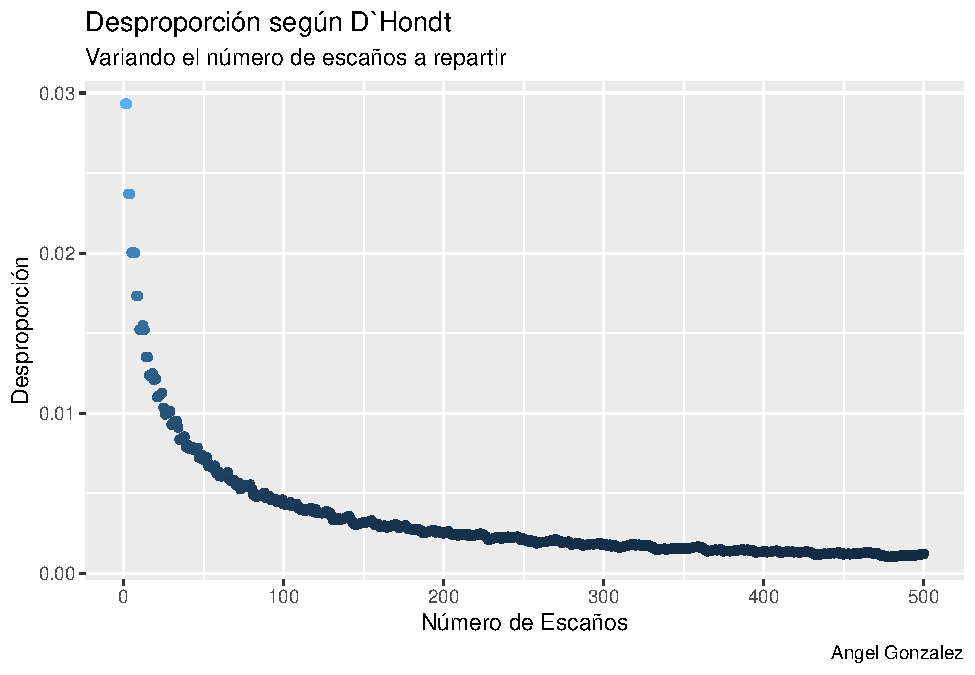
\includegraphics[width=1\linewidth]{figurasR/unnamed-chunk-5-1} \end{center}

\begin{center}\includegraphics[width=1\linewidth]{figurasR/unnamed-chunk-5-2} \end{center}

En estas primeras elecciones de 1977 podemos observar que la fuerza más
votada en las elecciones es el partido \emph{Unión de Centro
democrático} seguido del \emph{PSOE}. Observamos que según el método
vigente en España, el método D´Hondt, el partido \emph{UCD}, que ganaría
las elecciones, tendría una gran diferencia de votos respecto a los
demás partidos, por lo que facilitaría la gobernanza.

Comparando entre métodos de reparto observamos que el que más escaños da
a los partidos grandes es el método imperiali, que beneficia mucho a los
partidos más votados y penaliza mucho en escaños a los partidos tanto
medianos como poco votados. El método actual en España también tiene un
comportamiento similar al Imperiali aunque no tan acusado. En la otra
parte de la balanza encontramos al método Adams, el cual da muy pocos
escaños al partidos más votado y a los partidos medianos les beneficia.

En estas elecciones no se obtiene la mayoría absoluta en ningún método
excepto en el método Imperiali, en los demás métodos el partido ganador
debería de aliarse con uno o más partidos para obtener la mayoría
absoluta, los grandes perdedores en términos de escaños obtenidos son el
partido comunista y Alianza Popular, que podrían obtener hasta 10
escaños más de haber optado por otro método de reparto de votos.

\hypertarget{desproporciuxf3n}{%
\subsection{Desproporción}\label{desproporciuxf3n}}

\begin{center}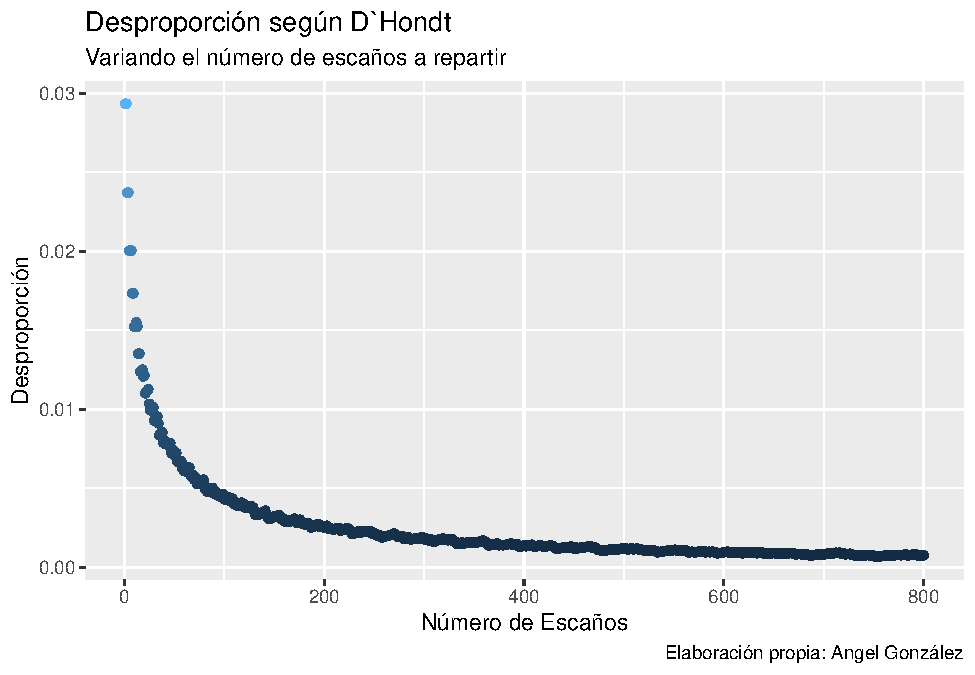
\includegraphics[width=1\linewidth]{figurasR/unnamed-chunk-6-1} \end{center}

\begin{center}\includegraphics[width=1\linewidth]{figurasR/unnamed-chunk-6-2} \end{center}

En el presente gráfico, en el que se mide la desproporción por
comunidades, observamos que en general entre todos los métodos las
comunidades más desproporcionadas son las ciudades de Ceuta y Melilla,
resultado lógico en tanto que al repartirse un único escaño es el
partido más votado únicamente el que obtiene el escaño. Es común entre
todos los métodos que la comunidad de Madrid sea la comunidad más
proporcionada, esto es debido a que es la comunidad en la que se
reparten más asientos y también la más poblada, por lo que cuando se
reparten los asientos por provincias, al utilizar el método D´Hondt,
como hemos visto beneficia a los lugares con más población.\\
En general los métodos que presentan una menor diferencia de
desproporción entre las distintas comunidades autónomas son el método
Danish, LR-Hare y el Saint-Lague, en cambio las que presentan una mayor
diferencia entre comunidades son el método Imperiali, Adams y el
Huntington-Hill.

Si nos centramos en el gráfico de la desproporción media según el método
de reparto podemos observar que la menor desproporción se encuentra en
los métodos LR-Hare, Danish y Sainte-Lague, mientras que la mayor
desproporción se encuentran en el método Imperiali y Adams. Especial
caso hacemos al método D´Hondt al ser el método utilizado actualmente en
España, observamos que ni es el mejor método ni tampoco es de los
peores, debido a ello sería conveniente cambiar el método de reparto a
otro mejor, que podría ser o bien el Sainte-Lague,LR-Hare o el Danish.

\hypertarget{auxf1o-1979}{%
\section{Año 1979}\label{auxf1o-1979}}

\hypertarget{comparativa-de-asientos-obtenidos-1}{%
\subsection{Comparativa de asientos
obtenidos}\label{comparativa-de-asientos-obtenidos-1}}

\begin{center}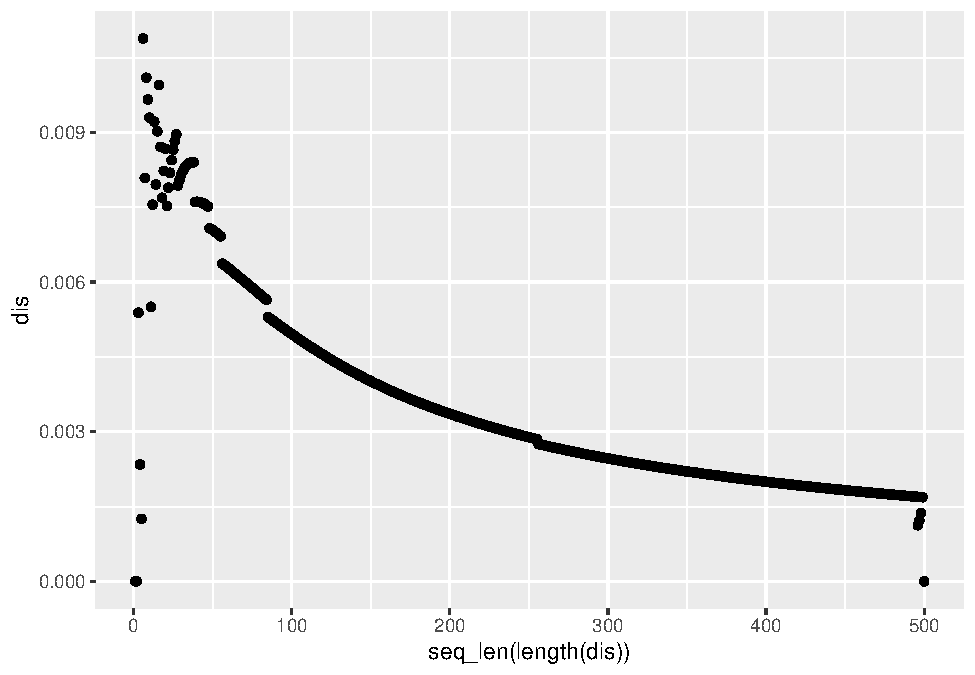
\includegraphics[width=1\linewidth]{figurasR/unnamed-chunk-8-1} \end{center}

\begin{center}\includegraphics[width=1\linewidth]{figurasR/unnamed-chunk-8-2} \end{center}

En estas elecciones de 1979 el partido más votado fué \emph{UCD} seguido
del \emph{PSOE}, según los distintos métodos de reparto únicamente en el
método Imperiali \emph{UCD} conseguiría la mayoría absoluta, en todos
los demás métodos de reparto no se alcanza la mayoría absoluta, los
partidos más castigados por utilizar el método D´Hondt son el partido
comunista y coalición Democrática, que podrían hasta doblar el número de
asientos obtenidos dependiendo del método de reparto que se haya
realizado. En estas elecciones podemos decir que hay dos grandes
partidos y dos medianos, UCD y el PSOE son los más grandes y el partido
comunista y coalición democrática son los partidos medianos, después ya
se encuentran todos los demás.

\hypertarget{desproporciuxf3n-1}{%
\subsection{Desproporción}\label{desproporciuxf3n-1}}

\begin{center}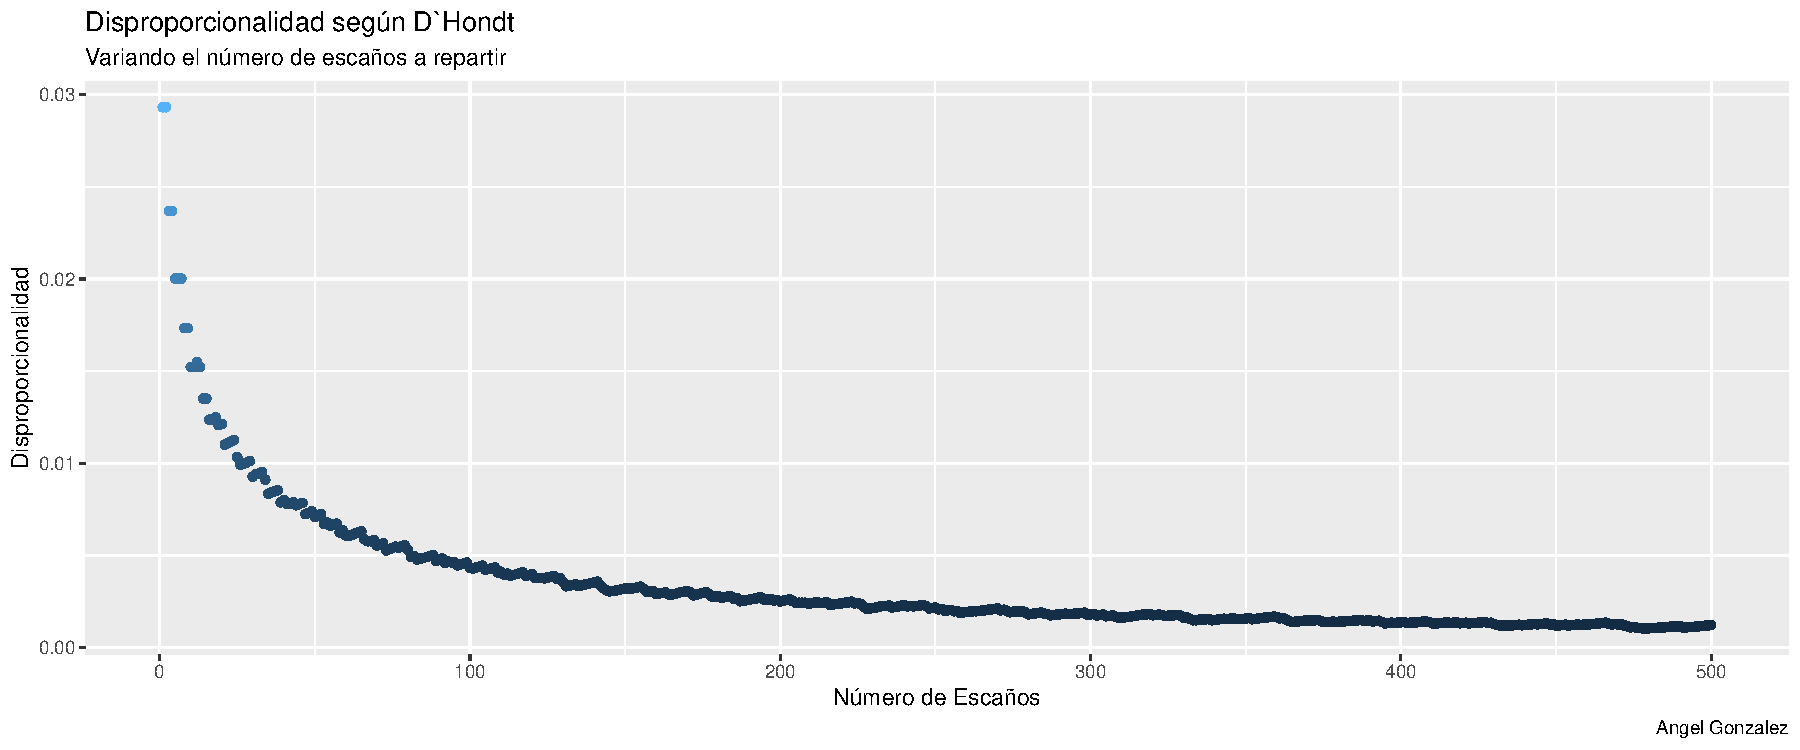
\includegraphics[width=1\linewidth]{figurasR/unnamed-chunk-9-1} \end{center}

\begin{center}\includegraphics[width=1\linewidth]{figurasR/unnamed-chunk-9-2} \end{center}

En el presente gráfico vemos como respecto a las anteriores elecciones
hay una mayor diferencia de desproporción entre comunidades, las
ciudades de Ceuta y Melilla siguen presentando la mayor desproporción
como es habitual y la comunidad de Madrid la menor desproporción. El
comportamiento de la desproporción en las comunidades se puede agrupar
en dos grupos, un grupo compuesto por los métodos Huntington-Hill y
Adams, y otro grupo con los restantes métodos.

Según la desproporción media los peores métodos de reparto se pueden
agrupar en tres, el método Imperiali, el Huntington-Hill, y el Adams, y
los mejores métodos de reparto en tres métodos, el LR-Hare, Danish y el
Sainte-Lague. En el caso del método D´Hondt se encuentra en un término
medio, por lo que sería conveniente cambiar el método de reparto a uno
más proporcional, que puede ser el Danish o el Sainte-Lague dentro de
los métodos de promedio mayor o bien por el LR-Hare de entre los métodos
de resto mayor.

\hypertarget{auxf1o-1982}{%
\section{Año 1982}\label{auxf1o-1982}}

\hypertarget{comparativa-de-asientos-obtenidos-2}{%
\subsection{Comparativa de asientos
obtenidos}\label{comparativa-de-asientos-obtenidos-2}}

\begin{center}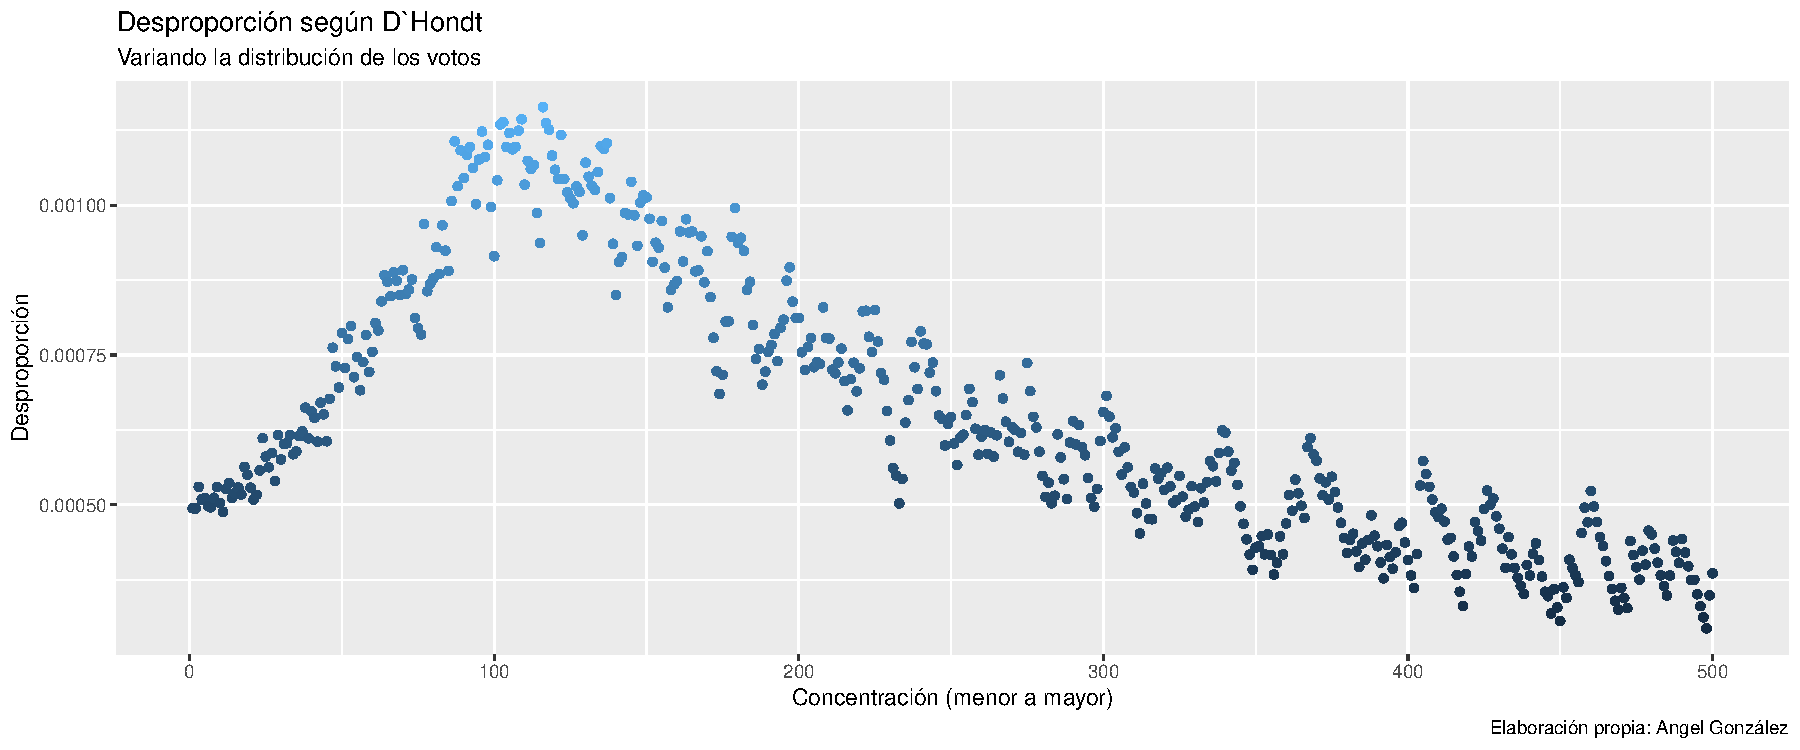
\includegraphics[width=1\linewidth]{figurasR/unnamed-chunk-11-1} \end{center}

\begin{center}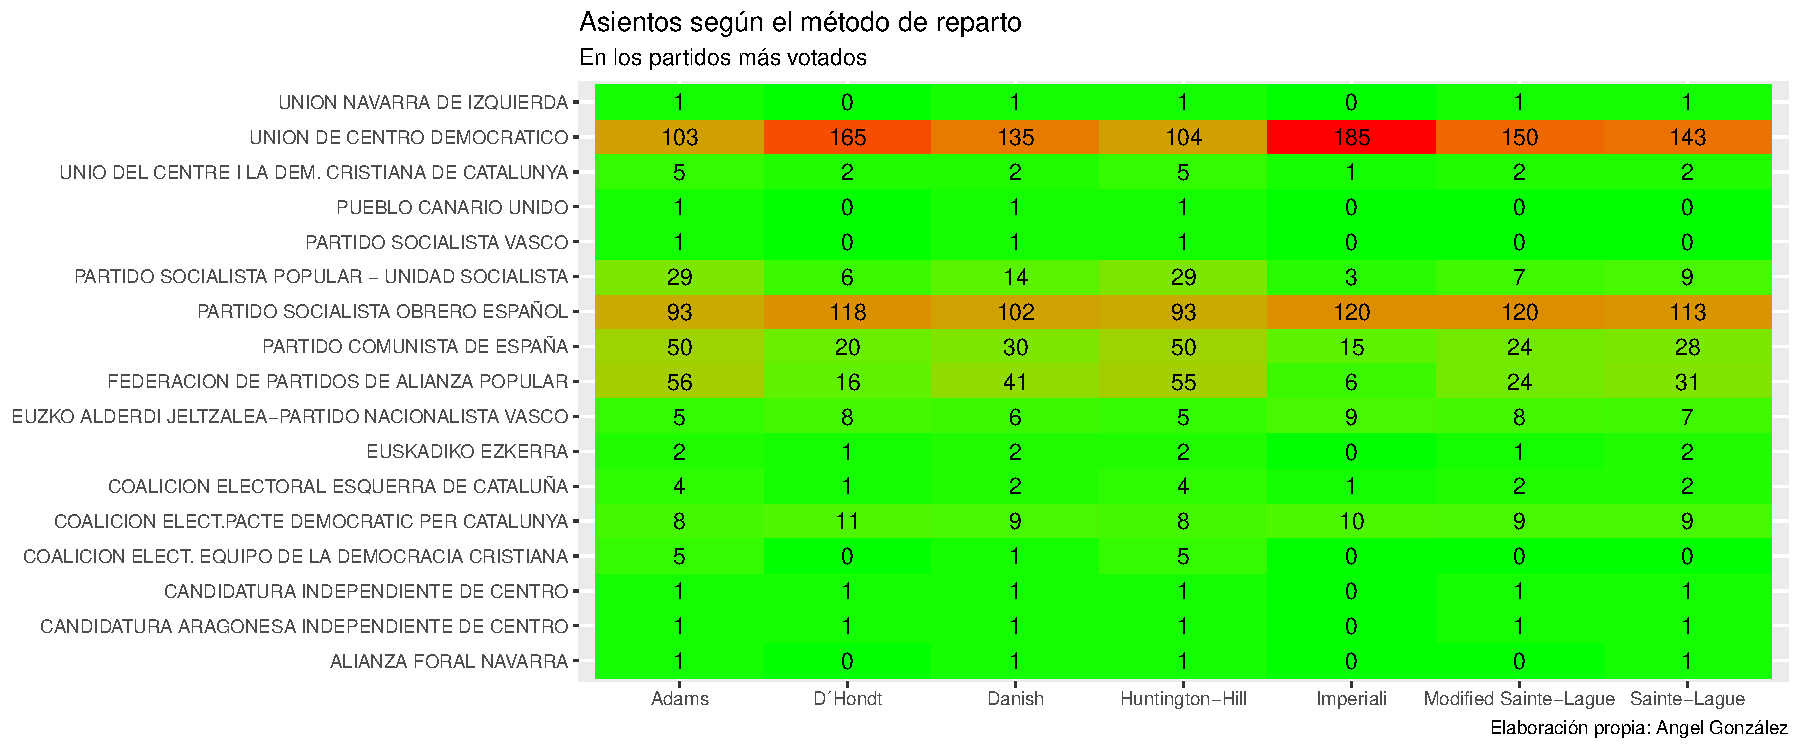
\includegraphics[width=1\linewidth]{figurasR/unnamed-chunk-11-2} \end{center}

En estas elecciones de 1982 el partido más votado es el \emph{PSOE} el
cual según la mayoría de los métodos de reparto, incluido el método
D´Hondt, alcanza la mayoría absoluta. Son unas elecciones en los que el
voto se concentra únicamente en dos partidos, que son el \emph{PSOE} y
\emph{Alianza Popular}, pero con una gran diferencia de asientos entre
ellos, donde el \emph{PSOE} casi dobla en escaños a \emph{Alianza
Popular}. El partido menos beneficiado en este año es \emph{UCD}, que
según el método D´Hondt obtendría 11 escaños mientras que si se optase
por otro método más proporcional como puede ser el método Danish o bien
el Sainte-Lague podría multiplicar sus escaños por 3 o 4.

\hypertarget{desproporciuxf3n-2}{%
\subsection{Desproporción}\label{desproporciuxf3n-2}}

\begin{center}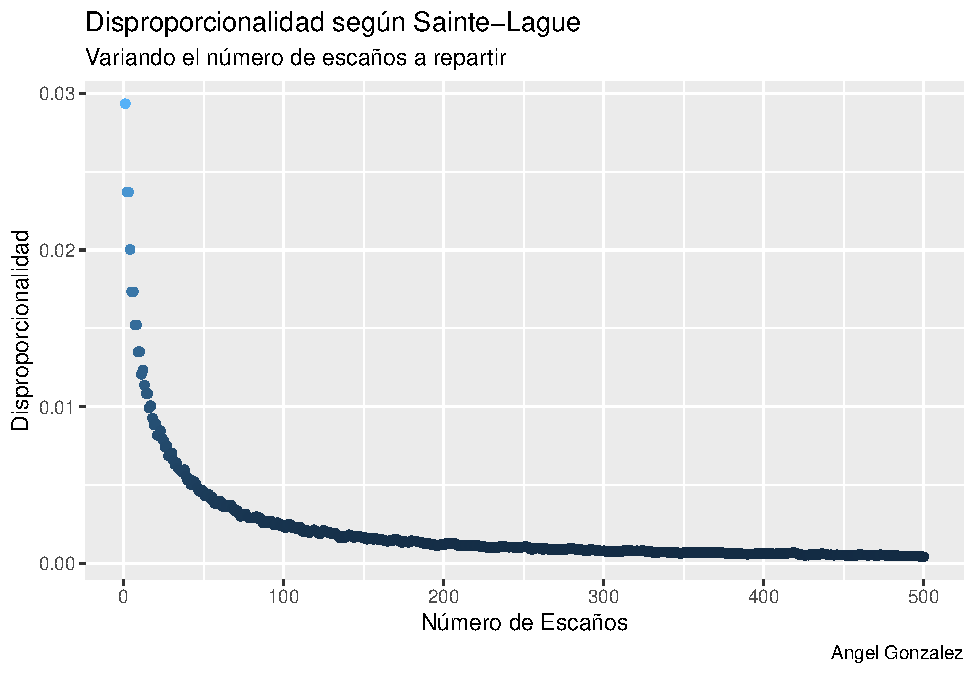
\includegraphics[width=1\linewidth]{figurasR/unnamed-chunk-12-1} \end{center}

\begin{center}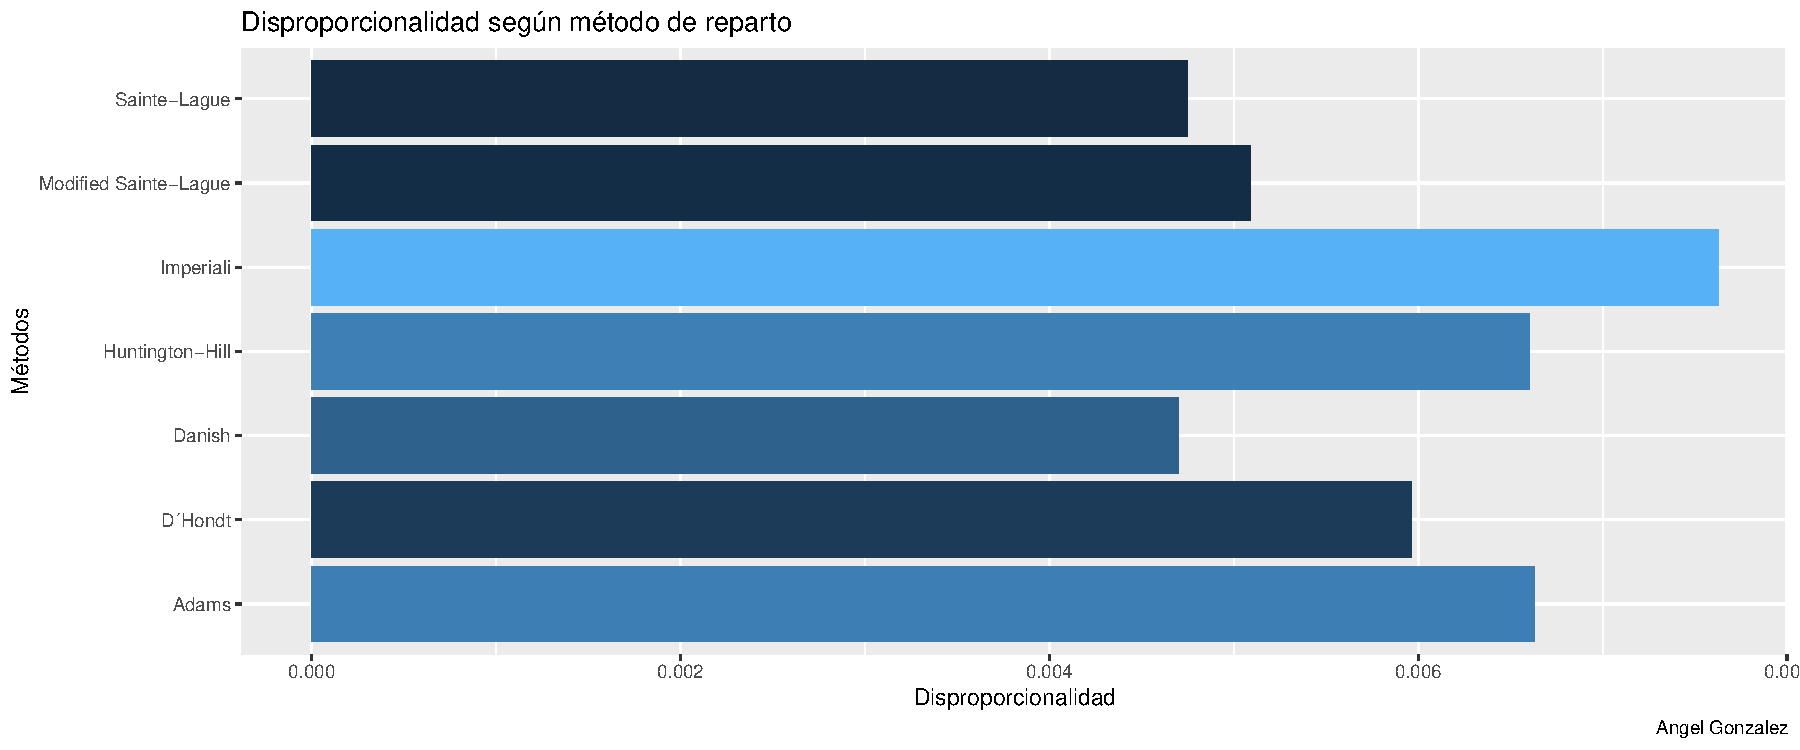
\includegraphics[width=1\linewidth]{figurasR/unnamed-chunk-12-2} \end{center}

Según la gráfica de desproporción por comunidades es un año en el que
generalmente no hay mucha diferencia de desproporción entre ellas, este
año las comunidades más desproporcionadas son la comunidad Foral de
Navarra y Cantabria sin contar las usuales de Ceuta y Melilla,mientras
que las comunidades más proporcionadas son la comunidad de Madrid y la
región de Murcia.

Según la desproporción media, se reconocen tres grupos distintos, un
grupo muy desproporcionado, con el método Adams como el más
desproporcionado, otro grupo medio en donde se encontraría el método
D´Hondt y un último grupo el cual sería el más proporcionado en el que
se encontraría el método Danish, LR-Hare y el Saint-Lague.

\hypertarget{auxf1o-1986}{%
\section{Año 1986}\label{auxf1o-1986}}

\hypertarget{comparativa-de-asientos-obtenidos-3}{%
\subsection{Comparativa de asientos
obtenidos}\label{comparativa-de-asientos-obtenidos-3}}

\begin{center}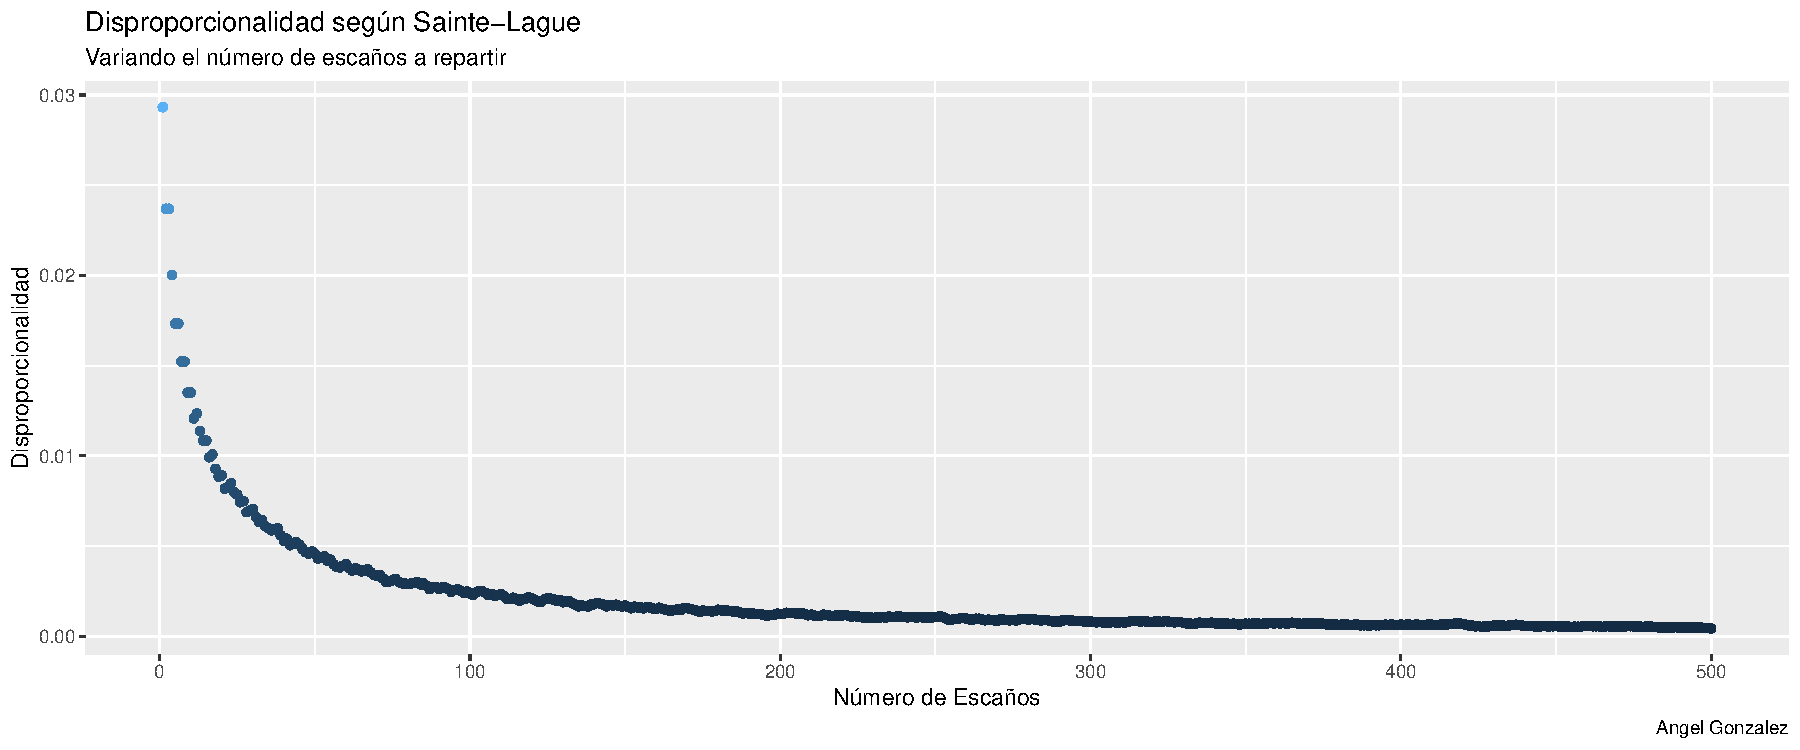
\includegraphics[width=1\linewidth]{figurasR/unnamed-chunk-14-1} \end{center}

\begin{center}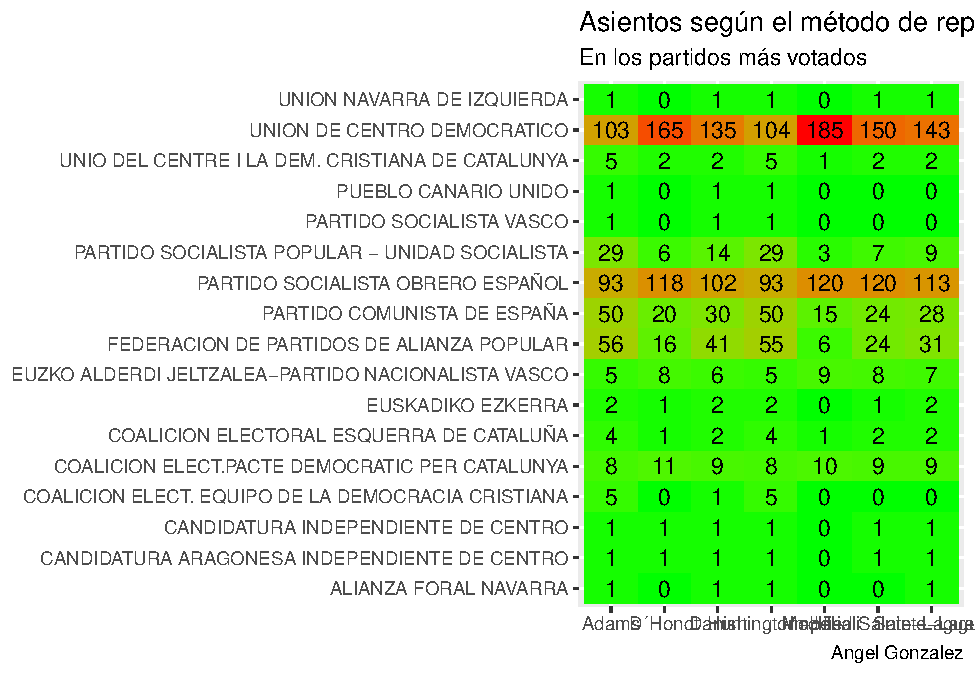
\includegraphics[width=1\linewidth]{figurasR/unnamed-chunk-14-2} \end{center}

En estas elecciones de 1986 el partido más votado fué el \emph{PSOE},
tal y como sucedió en las anteriores elecciones, son también unas
elecciones en donde hay únicamente dos partidos mayoritarios,
\emph{PSOE} y \emph{Coalición Popular}, ocurre en estas elecciones el
mismo escenario que en las anteriores elecciones, en donde el primer
partido casi dobla en escaños al segundo partido, aunque en este caso ya
se puede apreciar que la diferencia se va reduciendo entre los dos
grandes partidos, en general el PSOE alcanza la mayoría absoluta pero en
este año si utilizásemos los métodos más proporcionados es interesante
observar como perdería la mayoría absoluta tanto utilizando el método
Danish como el Sainte-Lague.\\
Este año también reconocemos un partido que podría decirse de nivel de
votos medio que queda muy dañado por el método de reparto D´Hondt, es el
partido \emph{Centro Democrático y Social}, el cual de utilizar los
métodos más proporcionados podría hasta duplicar sus escaños en el caso
de optar por el método Danish.

\hypertarget{desproporciuxf3n-3}{%
\subsection{Desproporción}\label{desproporciuxf3n-3}}

\begin{center}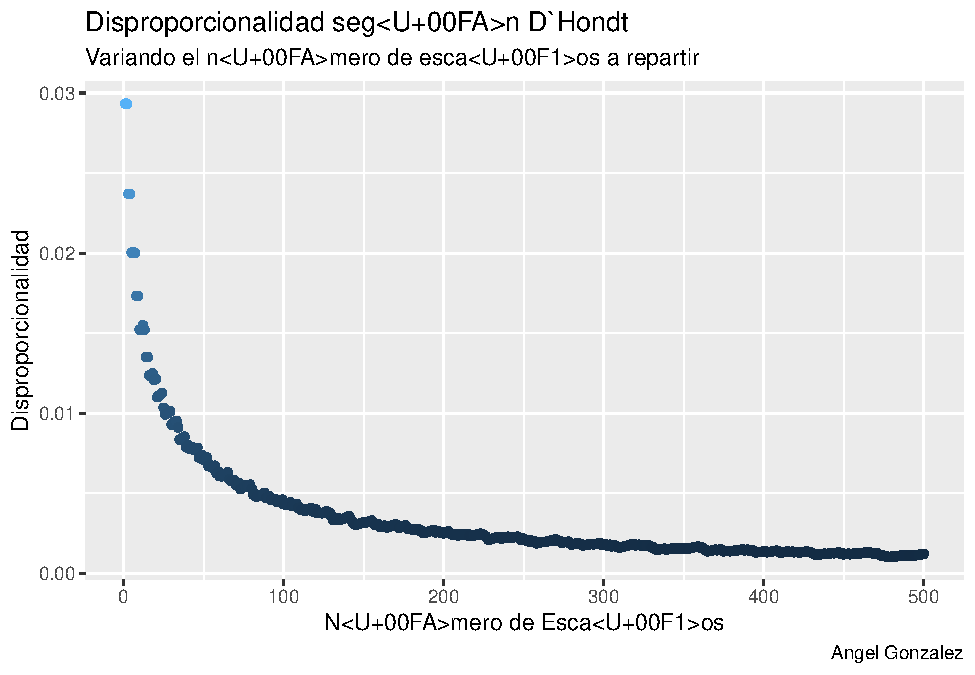
\includegraphics[width=1\linewidth]{figurasR/unnamed-chunk-15-1} \end{center}

\begin{center}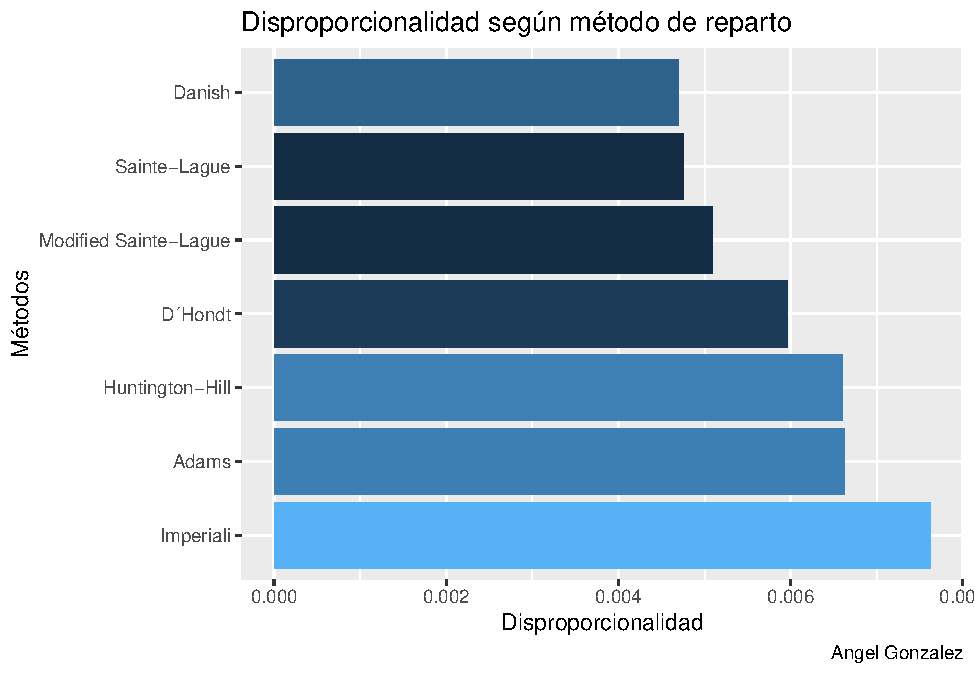
\includegraphics[width=1\linewidth]{figurasR/unnamed-chunk-15-2} \end{center}

Este año en el caso de la desproporción por comunidades podemos observar
que aumenta la diferencia respecto a las pasadas elecciones, una de las
comunidades más proporcionadas es la comunidad de Asturias mientras que
Aragón pasa a ser ahora una de las que más desproporción presenta. En
los extremos no hay novedades, Madrid sigue siendo la más proporcionada
y las ciudades de Ceuta y Melilla las que menos proporcionadas resultan.

Según el método de reparto este año el método Imperiali es el más
desproporcionado con una gran diferencia respecto a los restantes
métodos, los demás métodos se sitúan en un mismo grupo, en donde los
métodos más proporcionados este año son los métodos LR-Hare y Danish
seguido muy de cerca por el Sainte-Lague.

\hypertarget{auxf1o-1989}{%
\section{Año 1989}\label{auxf1o-1989}}

\hypertarget{comparativa-de-asientos-obtenidos-4}{%
\subsection{Comparativa de asientos
obtenidos}\label{comparativa-de-asientos-obtenidos-4}}

\begin{center}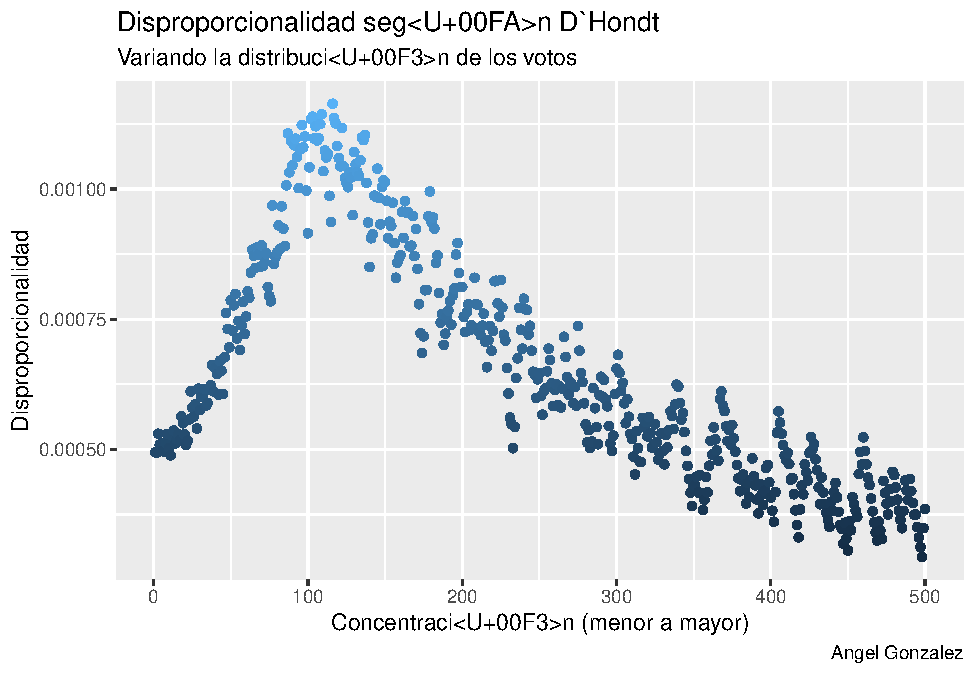
\includegraphics[width=1\linewidth]{figurasR/unnamed-chunk-17-1} \end{center}

\begin{center}\includegraphics[width=1\linewidth]{figurasR/unnamed-chunk-17-2} \end{center}

En estas elecciones de 1989 el partido más votado es, como sucedió el
las anteriores elecciones, el \emph{PSOE}, vemos como aparece por
primera vez el \emph{Partido Popular} como segunda fuerza tomando el
puesto que antes tenía \emph{Coalición Popular}, estas elecciones
también son muy bipartidistas aunque se va debilitando ese bipartidismo,
ahora podemos decir que hay dos partidos hegemónicos, PSOE y PP, y tres
partidos medianos, los cuales serían el Centro Democrático y Social,
Izquierda Unida y Convergencia y Unión, de todos estos partidos los más
desfavorecidos por la utilización del método D´Hondt son IU y Centro
Democrático, los cuales de haber utilizado los métodos más
proporcionales podrían hasta duplicar su presencia en el congreso. Por
la otra parte en el caso del PSOE pasaría de alcanzar la mayoría
absoluta justa con 175 escaños a perder la mayoría absoluta en el caso
de optar por los métodos más proporcionales.

\hypertarget{desproporciuxf3n-4}{%
\subsection{Desproporción}\label{desproporciuxf3n-4}}

\begin{center}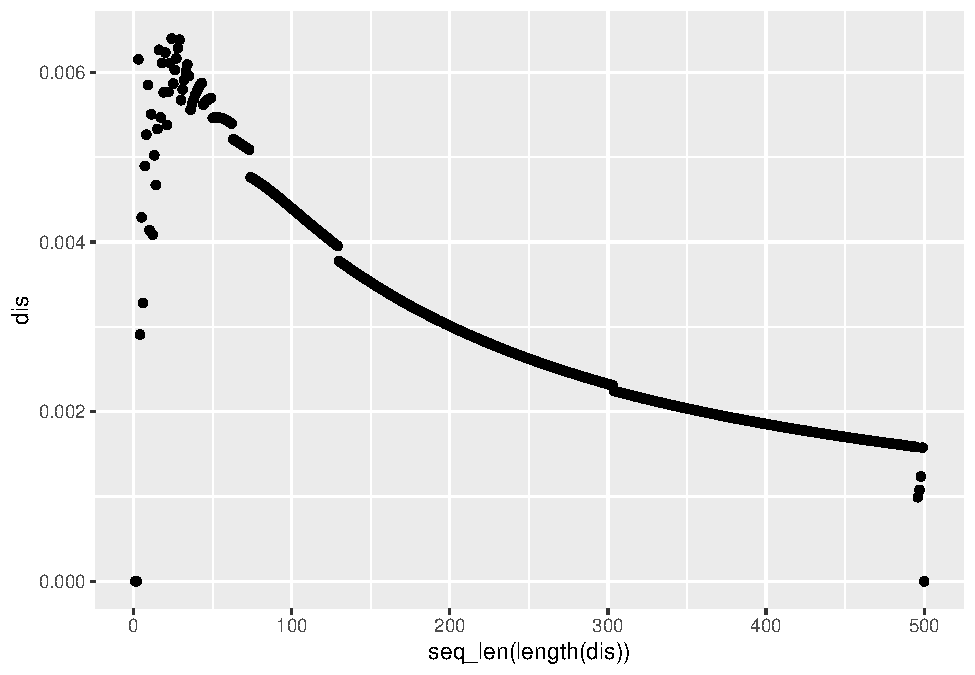
\includegraphics[width=1\linewidth]{figurasR/unnamed-chunk-18-1} \end{center}

\begin{center}\includegraphics[width=1\linewidth]{figurasR/unnamed-chunk-18-2} \end{center}

Este año aumenta ligeramente la diferencia de desproporción entre
comunidades, sin encontrar novedades en las comunidades más
proporcionales, Madrid, y las más desproporcionadas, las ciudades de
Ceuta y Melilla. Observando los métodos de reparto hay dos grupos
diferenciados, uno en el que se encuentran el método Adams, LR-Imperiali
y el método de Huntington-Hill, en los cuales no se encuentran
comunidades con picos de desproporción pero por el lado contrario su
desproporción media es alta, y otro grupo que serían los restantes
métodos los cuales todos presentan unos mismos picos máximos como
míninos.

Estas elecciones de 1989 la desproporción media se agrupa en tres
grupos, de alta, media y baja desproporción, el más desproporcionado
vuelve a ser el método Imperiali, el método D´Hondt sigue en el grupo
medio y el método más proporcionado vuelve a ser el Danish aunque le
sigue muy cerca el método Sainte-Lague.

\hypertarget{auxf1o-1993}{%
\section{Año 1993}\label{auxf1o-1993}}

\hypertarget{comparativa-de-asientos-obtenidos-5}{%
\subsection{Comparativa de asientos
obtenidos}\label{comparativa-de-asientos-obtenidos-5}}

\begin{center}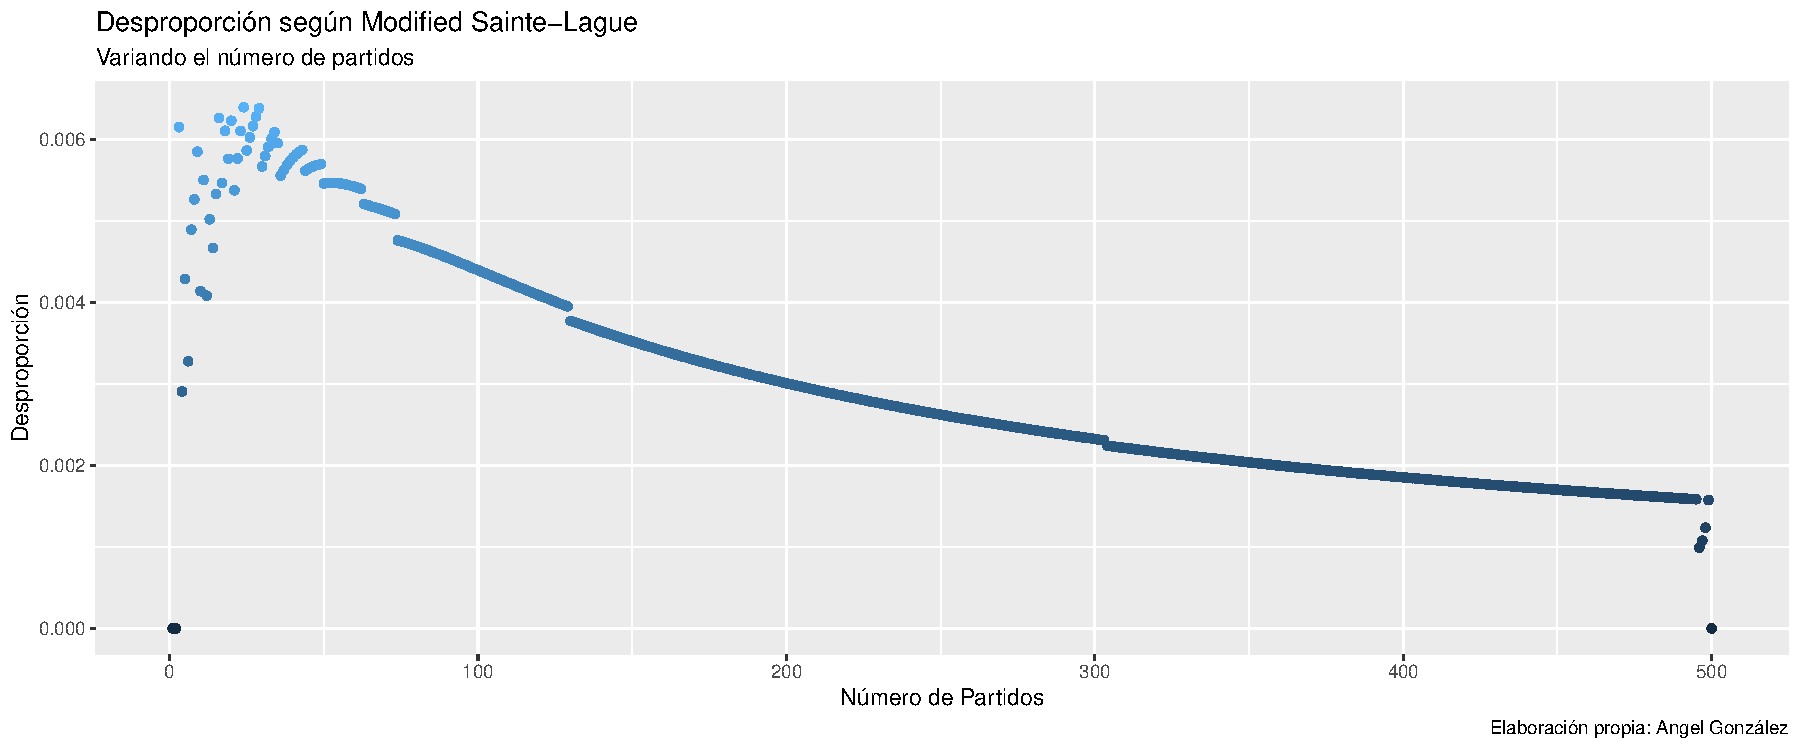
\includegraphics[width=1\linewidth]{figurasR/unnamed-chunk-20-1} \end{center}

\begin{center}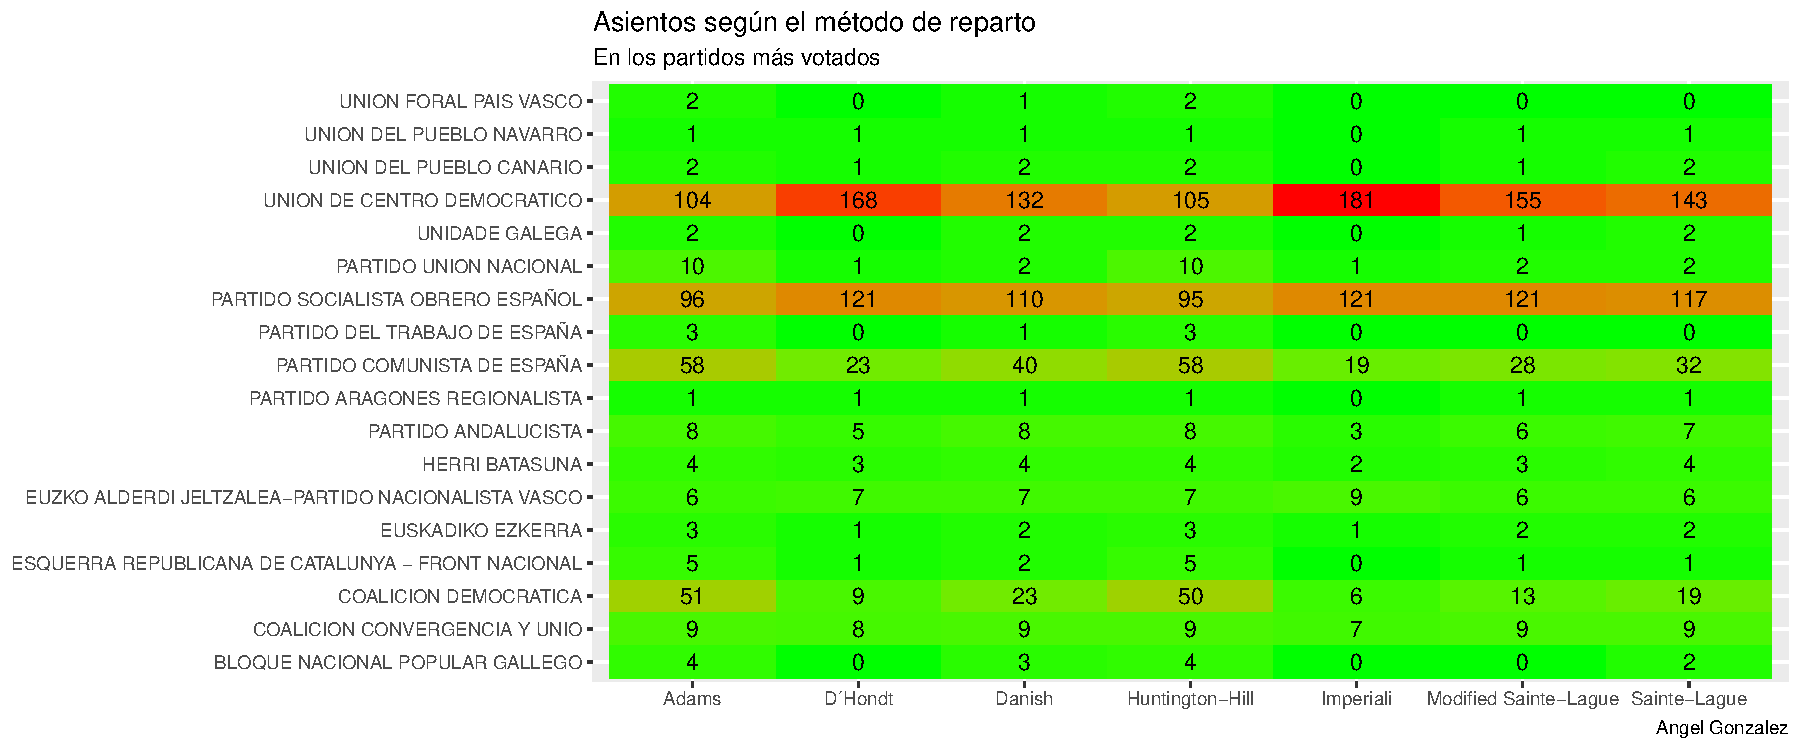
\includegraphics[width=1\linewidth]{figurasR/unnamed-chunk-20-2} \end{center}

En las elecciones de 1993 podemos observar como la fuerza del primer
partido va decreciendo lentamente. Los dos partidos más votados son el
\emph{PSOE} y el \emph{PP} respectivamente, la diferencia estas
elecciones es que el PSOE ha perdido la mayoría absoluta según el método
D´Hondt y en cambio el \emph{PP} ha aumentado su presencia
significativamente y está ya relativamente cerca de alcanzar al
\emph{PSOE}. De haber utilizado los métodos más proporcionales
resultaría en una menor diferencia de escaños entre estos dos grandes
partidos, el partido más castigado en estas elecciones sigue siendo
\emph{IU}, el cual podría haber obtenido de 1.5 a 2 veces más asientos
de haber cambiado de método de reparto. Son unas elecciones en donde hay
dos partidos hegemónicos y dos partidos medianos que son \emph{IU} y
\emph{CIU}, como hemos visto \emph{IU} es un partido muy castigado por
el método de reparto actual, en cambio \emph{CIU} no se vería agraviado
o beneficiado al cambiar el método de reparto.

\hypertarget{desproporciuxf3n-5}{%
\subsection{Desproporción}\label{desproporciuxf3n-5}}

\begin{center}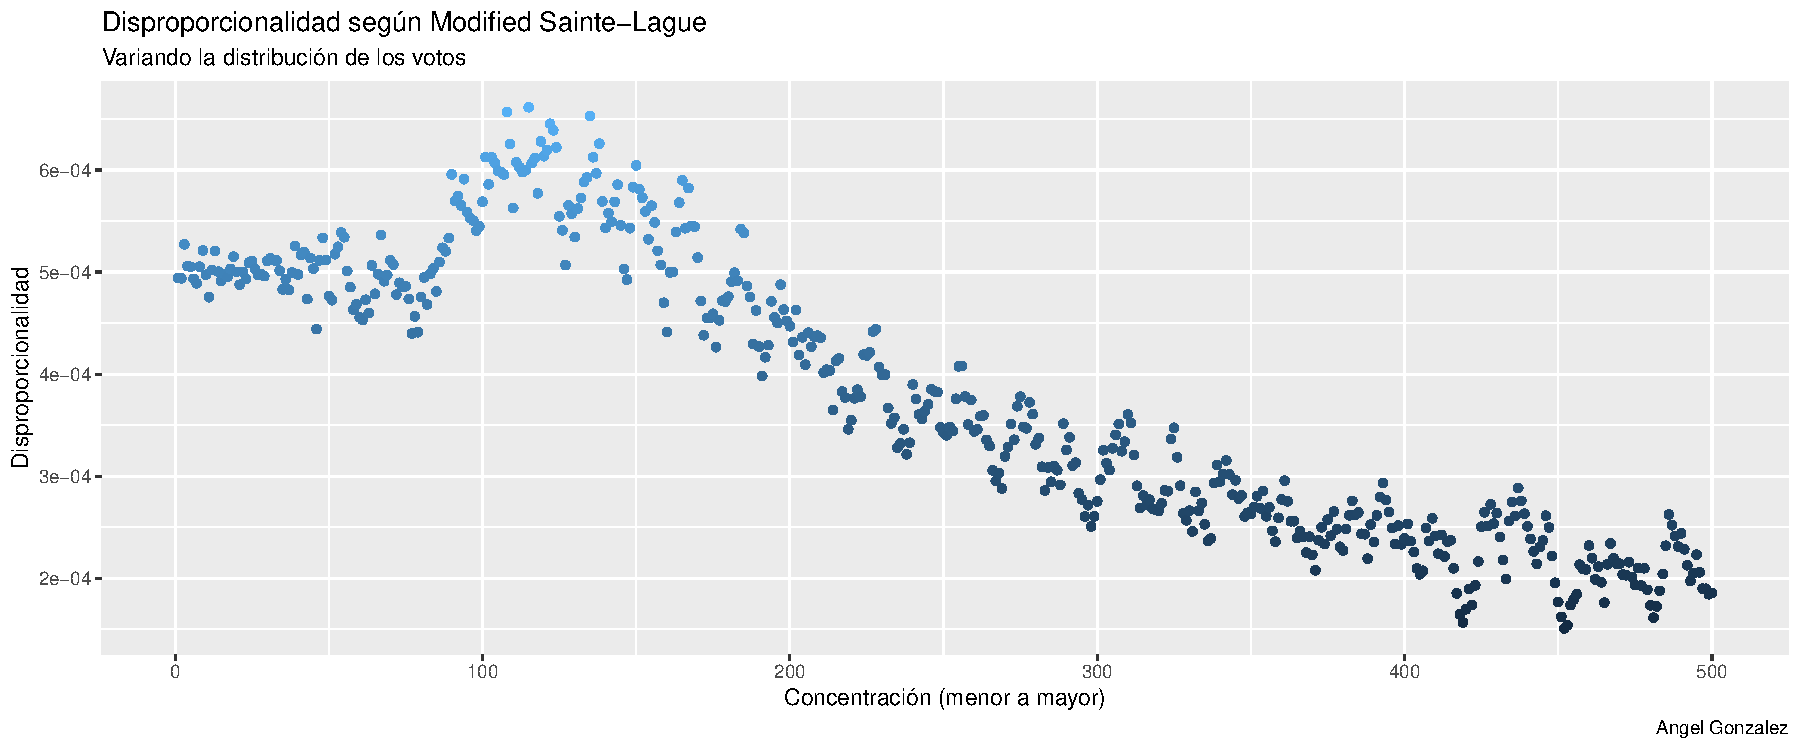
\includegraphics[width=1\linewidth]{figurasR/unnamed-chunk-21-1} \end{center}

\begin{center}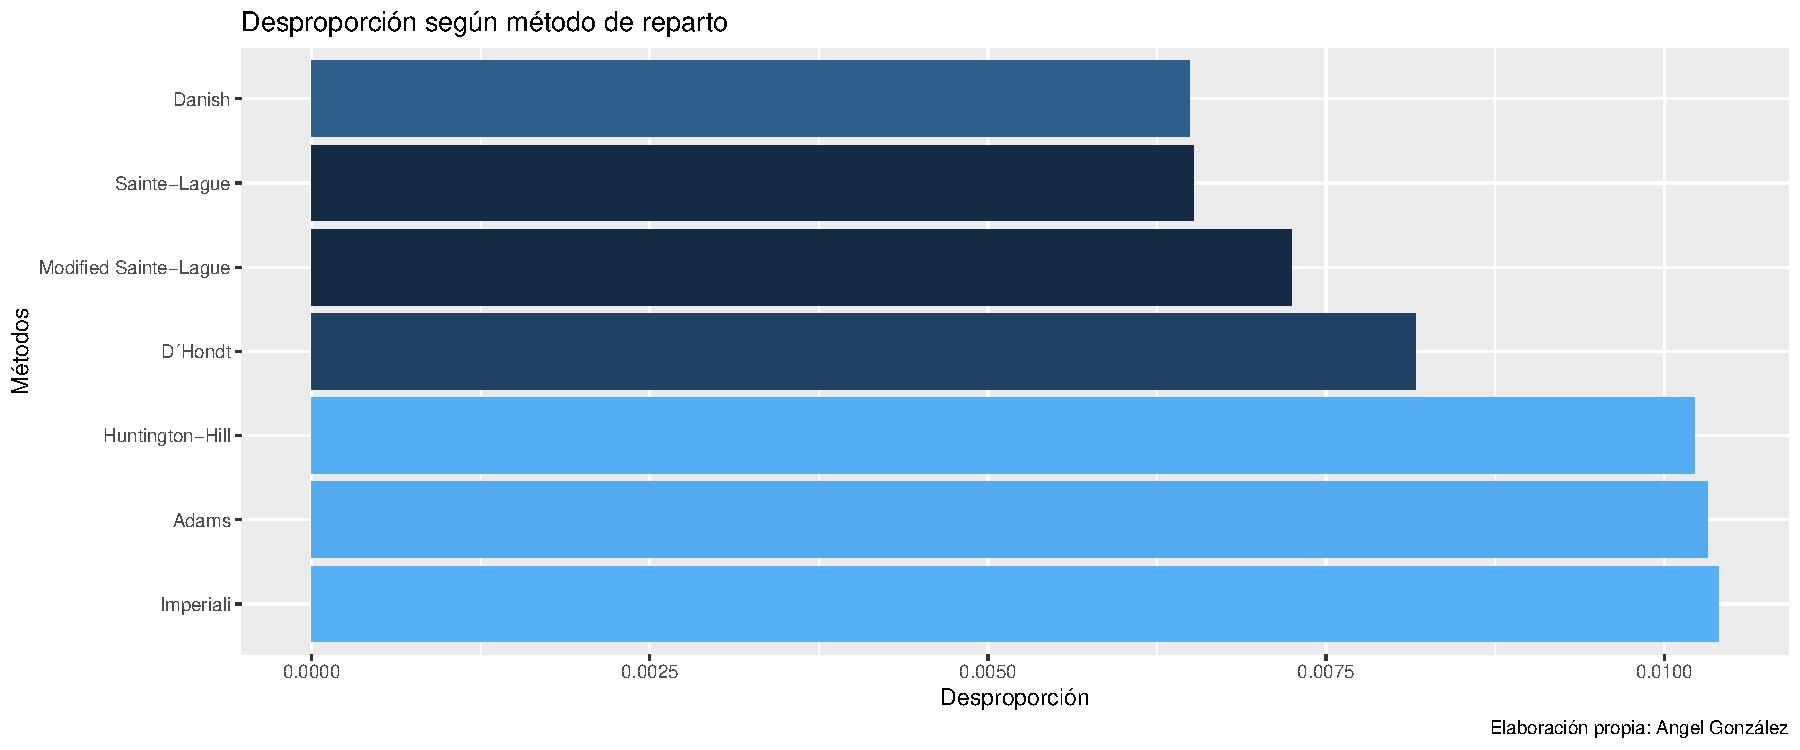
\includegraphics[width=1\linewidth]{figurasR/unnamed-chunk-21-2} \end{center}

En estas elecciones se observan más picos de desproporción en
comparación con las elecciones anteriores, especialmente aumenta su
desproporción el Pais Vasco y Aragón, no hay novedades en los máximos ni
en los mínimos. Siguen dos grupos con un comportamiento similar, en un
grupo los métodos de Adams, Huntington-Hill y LR-Imperiali y los
restantes en el otro grupo.

Este año en el caso de la desproporción media según el método de reparto
vemos que hay diferencias en los métodos más desproporcionales,
usualmente el método más desproporcionado ha sido el Imperiali, en estas
elecciones esto cambia, de hecho mejora en dos puestos. Los más
desproporcionados este año entonces son los métodos Adams y de
Huntington-Hill, en el caso de los más proporcionados no hay novedades,
siguen siendo los métodos LR-Hare y Danish seguido muy de cerca por el
Sainte-Lague.

\hypertarget{auxf1o-1996}{%
\section{Año 1996}\label{auxf1o-1996}}

\hypertarget{comparativa-de-asientos-obtenidos-6}{%
\subsection{Comparativa de asientos
obtenidos}\label{comparativa-de-asientos-obtenidos-6}}

\begin{center}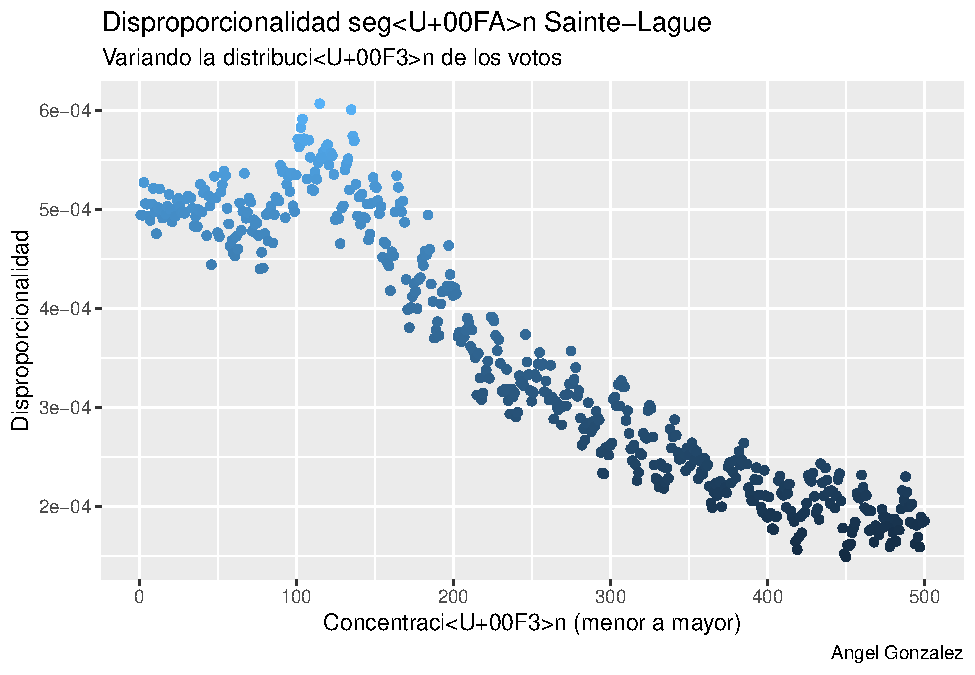
\includegraphics[width=1\linewidth]{figurasR/unnamed-chunk-23-1} \end{center}

\begin{center}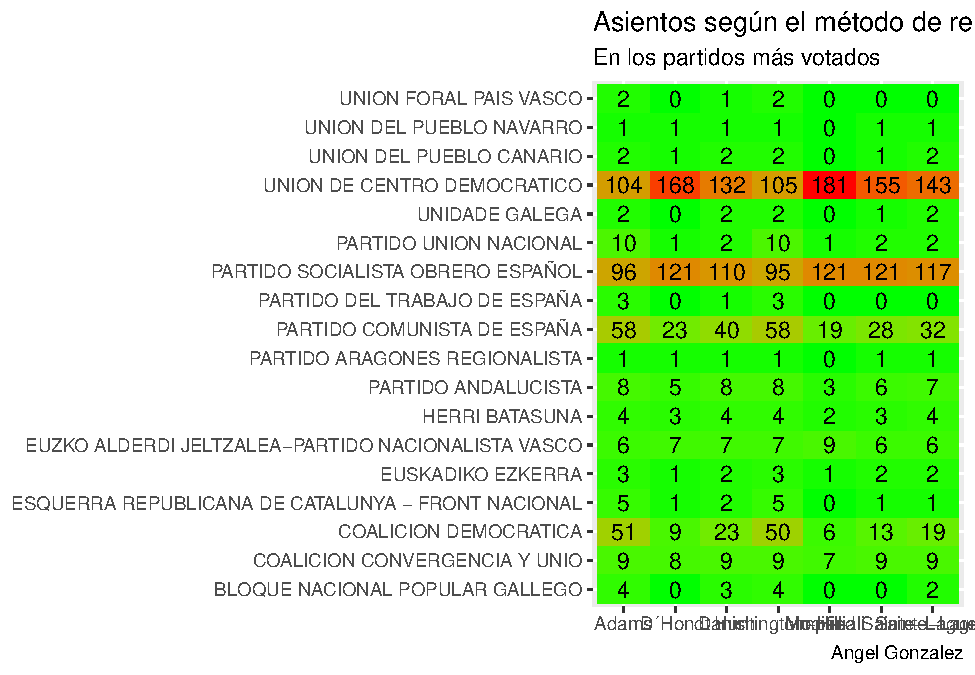
\includegraphics[width=1\linewidth]{figurasR/unnamed-chunk-23-2} \end{center}

En estas elecciones de 1996 son las primeras elecciones en donde el
\emph{PP} son la fuerza más votada, el \emph{PSOE} que ya llevaba una
tendencia descendiente a lo largo de las últimas elecciones al final
pierde el primer puesto a favor del \emph{PP}. Sigue presentandose un
bipartidismo significativo, seguidamente de dos partidos medianos,
todavía el PP a pesar de ganar las elecciones no alcanza la mayoría
absoluta en ninguno de los métodos analizados. Izquierda Unida sigue
siendo el partido más castigado, podría duplicar el número de escaños de
haber escogido otro método más proporcional.

\hypertarget{desproporciuxf3n-6}{%
\subsection{Desproporción}\label{desproporciuxf3n-6}}

\begin{center}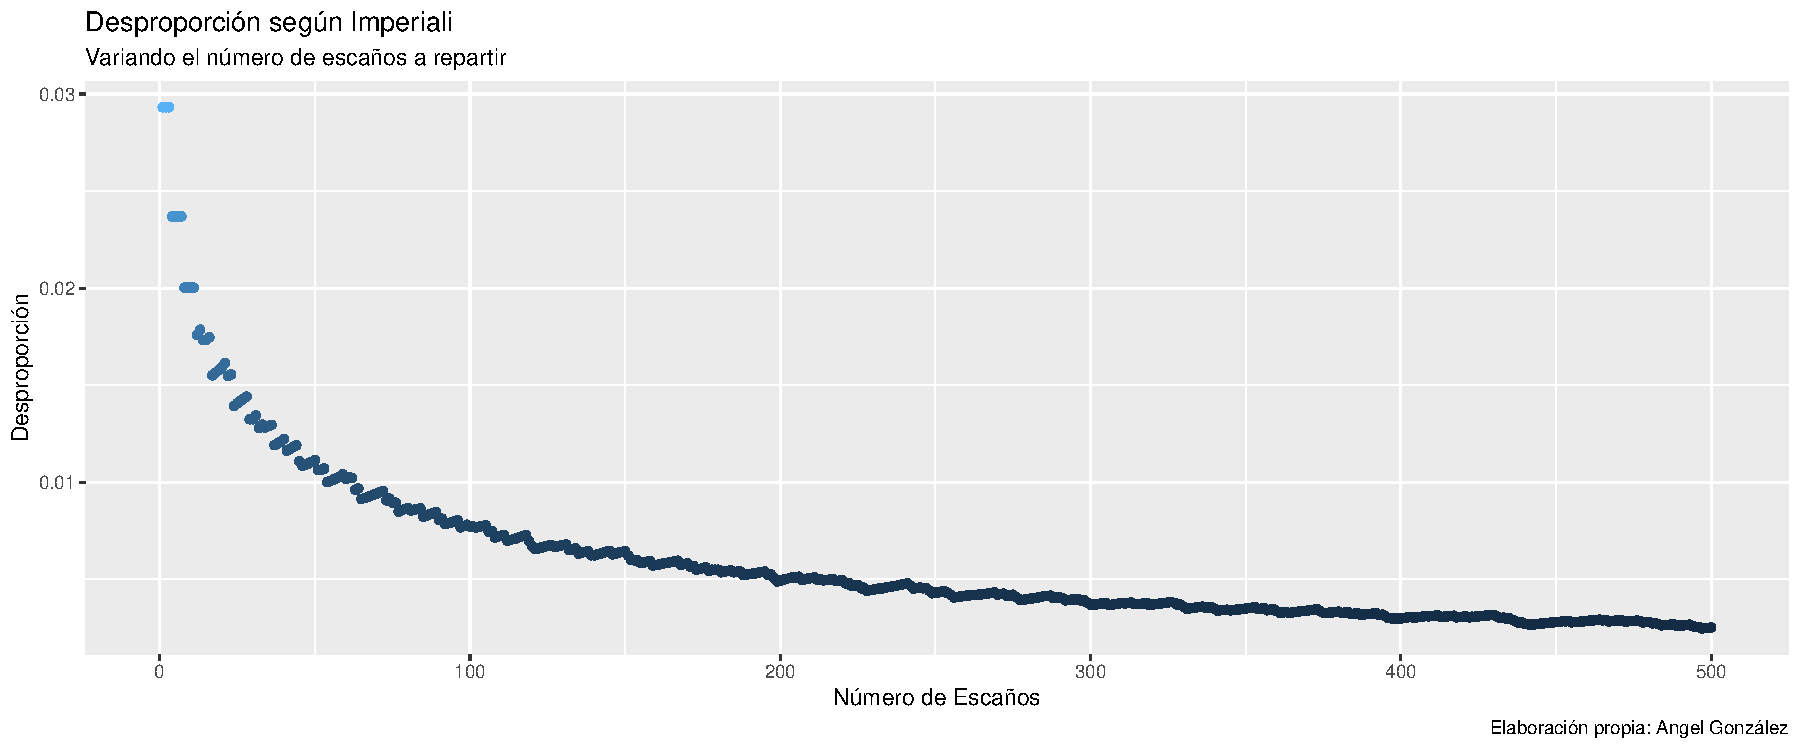
\includegraphics[width=1\linewidth]{figurasR/unnamed-chunk-24-1} \end{center}

\begin{center}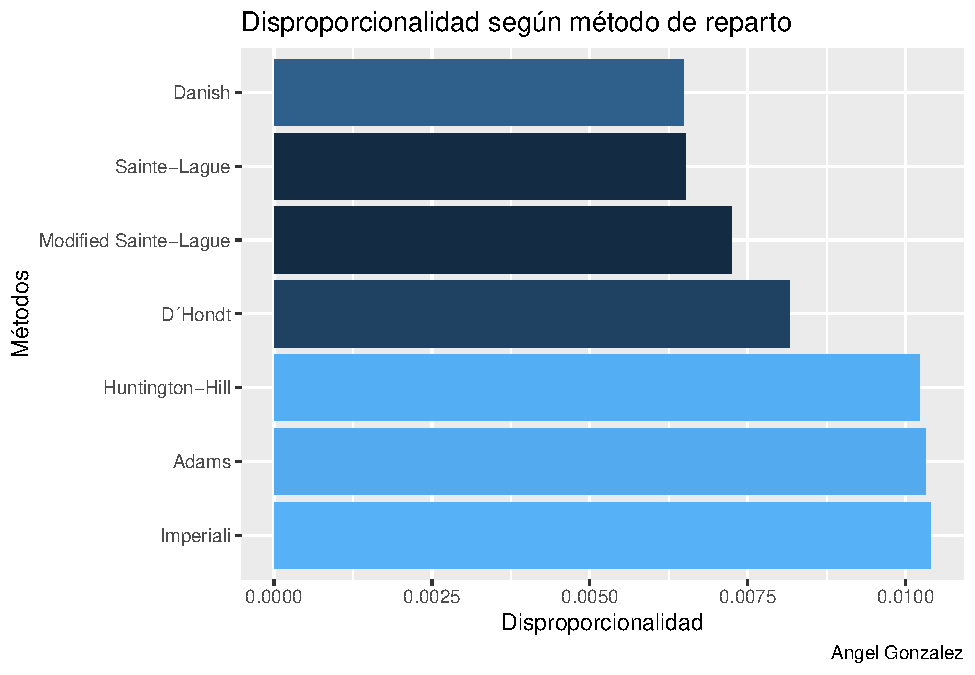
\includegraphics[width=1\linewidth]{figurasR/unnamed-chunk-24-2} \end{center}

En estas elecciones de 1996 se observa una desproporción similar a las
elecciones anteriores, en este año el comportamiento de la desproporción
por provincias se puede agrupar en tres grupos, uno en el que estaría el
método LR-Imperiali, con una desproporción muy marcada en la comunidad
Foral de Navarra, otro en los que estarían los métodos Adams y
Huntington-Hill, y el tercero con los métodos restantes.

Este año en el caso de la desproporción media según el método de reparto
vemos que hay diferencias en los métodos con más desproporción respecto
a la anterior elección, el método más desproporcionado vuelve a ser el
Imperiali. En el caso de los más proporcionados cambia también, el
método Danish pasa a un cuarto puesto superado por el método
Sainte-Lague, los mejores son el método LR-Imperiali y LR-Hare. Los más
desproporcionados este año son el método anteriormente citado,
Imperiali, seguido muy de cerca por los métodos Adams y de
Huntington-Hill, .

\hypertarget{auxf1o-2000}{%
\section{Año 2000}\label{auxf1o-2000}}

\hypertarget{comparativa-de-asientos-obtenidos-7}{%
\subsection{Comparativa de asientos
obtenidos}\label{comparativa-de-asientos-obtenidos-7}}

\begin{center}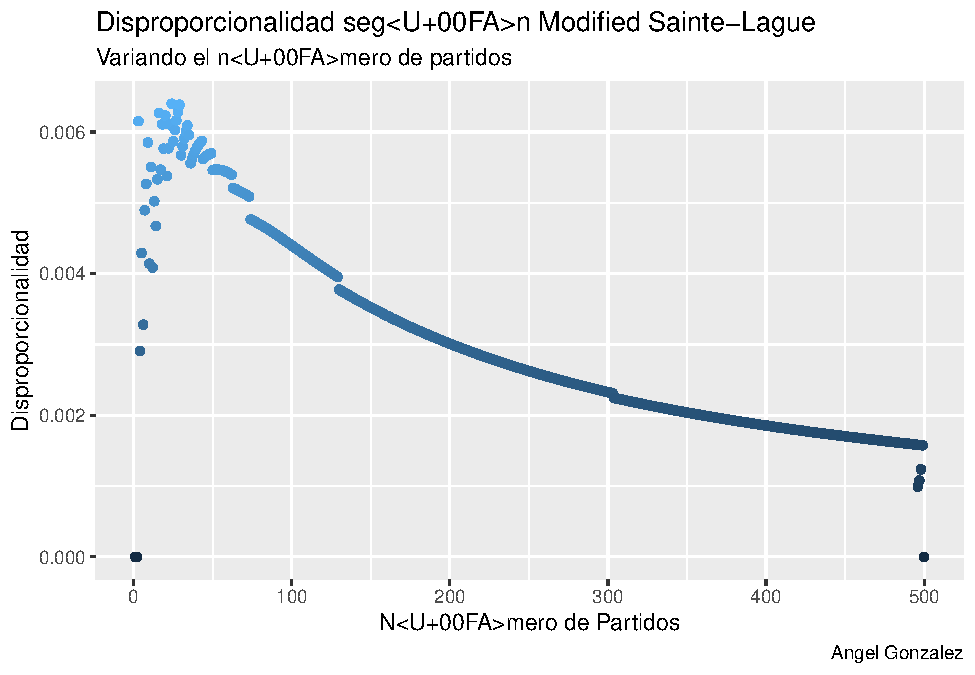
\includegraphics[width=1\linewidth]{figurasR/unnamed-chunk-26-1} \end{center}

\begin{center}\includegraphics[width=1\linewidth]{figurasR/unnamed-chunk-26-2} \end{center}

En las elecciones del año 2000 el partido más votado vuelve a ser el
\emph{Partido Popular} seguido del \emph{PSOE}, en estas elecciones
según el método D´Hondt utilizado en España el \emph{PP} conseguiría una
mayoría absoluta holgada, es una elección con un claro bipartidismo
donde se podría decir que no existen partidos medianos. Si optásemos por
otro método de reparto más proporcional como puede ser el método Danish
o el Sainte-Lague el PP alcanzaría la mayoría absoluta o se quedaría a
muy pocos escaños de alcanzarla, en cambio veríamos a muchos partidos
pequeños con menos de tres votos casi duplicar su presencia en escaños.
El partido más castigado por utilizar el método D´Hondt en estas
elecciones sigue siendo Izquierda Unida.

\hypertarget{desproporciuxf3n-7}{%
\subsection{Desproporción}\label{desproporciuxf3n-7}}

\begin{center}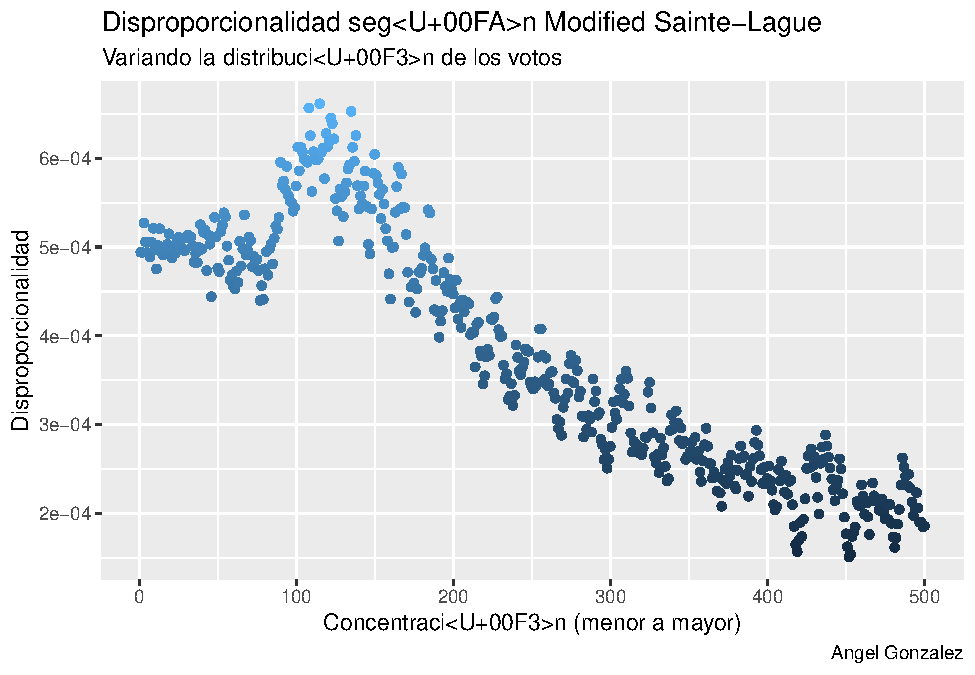
\includegraphics[width=1\linewidth]{figurasR/unnamed-chunk-27-1} \end{center}

\begin{center}\includegraphics[width=1\linewidth]{figurasR/unnamed-chunk-27-2} \end{center}

Observando la desproporción por comunidades tanto el método Adams como
el Huntington-Hill tienen un comportamiento diferente respecto a los
demás, siguen siendo los más desproporcionados las ciudades de Ceuta y
Melilla, y la más proporcionada la Comunidad de Madrid, este año es
especialmente alta la desproporción de las Islas Baleares respecto a
anteriores elecciones.

Si miramos la gráfica de la desproporción según el método de reparto se
pueden agrupar los métodos en dos grupos, uno con gran desproporción en
el que estarían incluidos los métodos Adams, Imperiali y
Huntington-Hill, y el otro grupo restante con una desproporción media
baja. Seguimos observando que el método D´Hont no es el mejor aunque en
estas elecciones se puede considerar un método aceptable siendo los
mejores el método LR-Hare, Danish y Saint-Lague, todos ellos con una
desproporción muy similar.

\hypertarget{auxf1o-2004}{%
\section{Año 2004}\label{auxf1o-2004}}

\hypertarget{comparativa-de-asientos-obtenidos-8}{%
\subsection{Comparativa de asientos
obtenidos}\label{comparativa-de-asientos-obtenidos-8}}

\begin{center}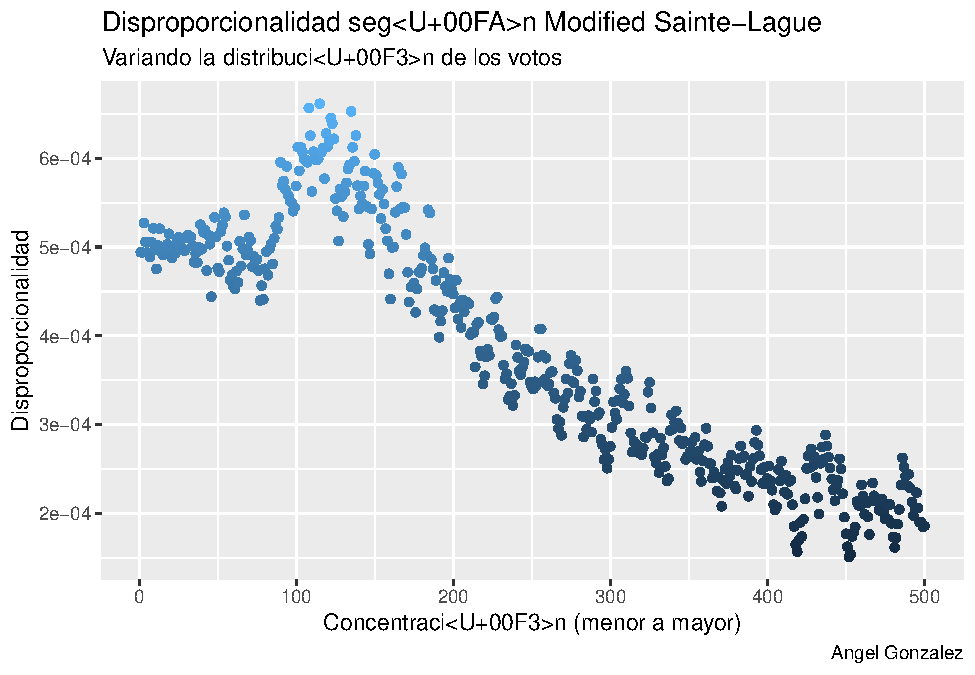
\includegraphics[width=1\linewidth]{figurasR/unnamed-chunk-29-1} \end{center}

\begin{center}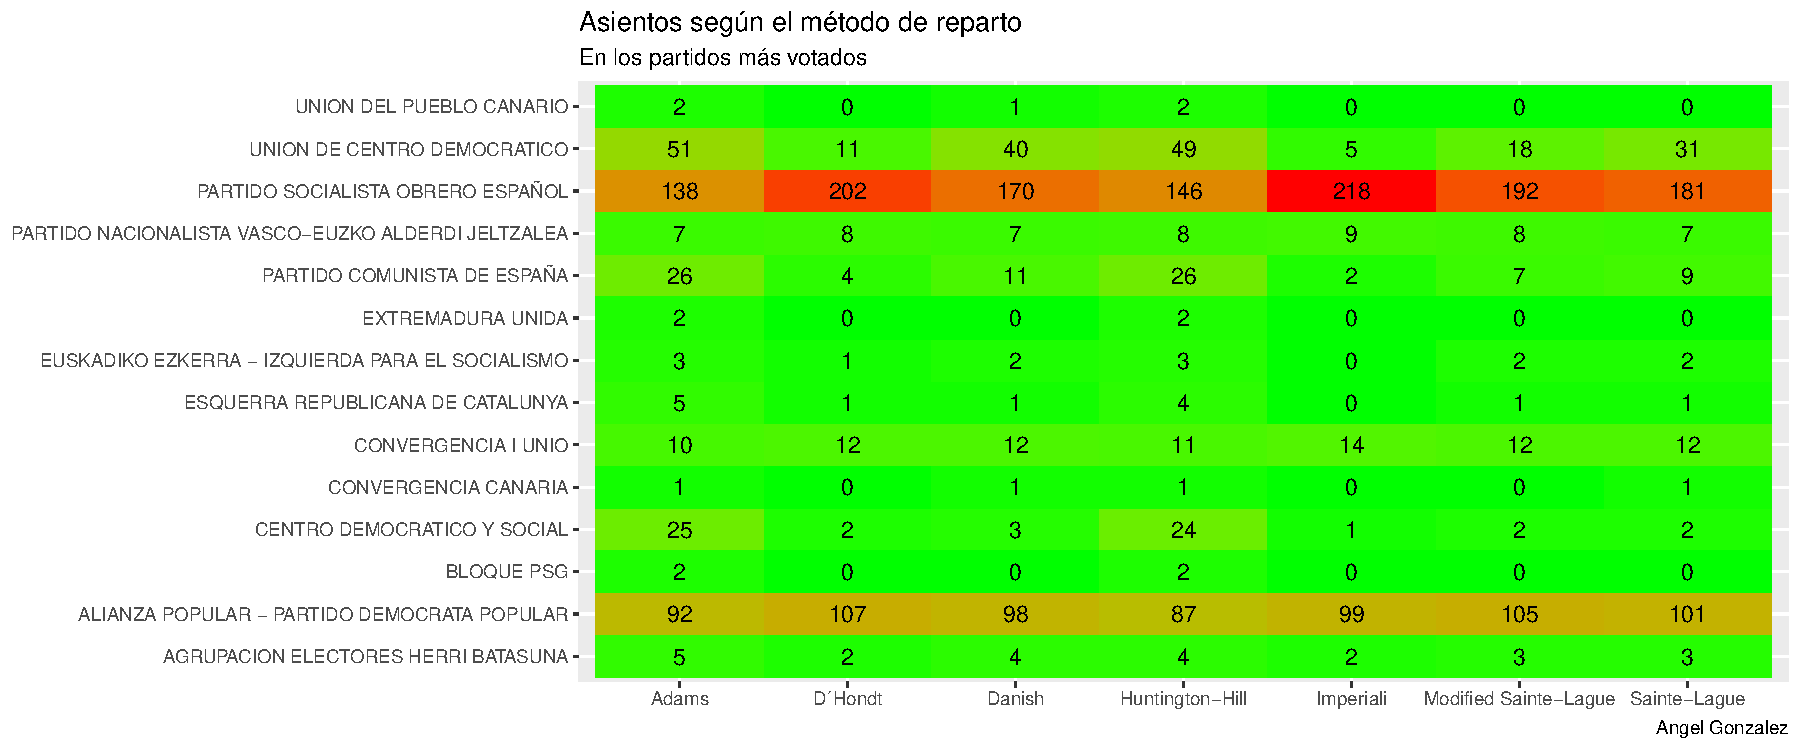
\includegraphics[width=1\linewidth]{figurasR/unnamed-chunk-29-2} \end{center}

En estas elecciones del año 2004 volvemos a ver unas elecciones con un
claro bipartidismo y con una diferencia de escaños entre partidos cada
vez menor, en estas elecciones el partido más votado cambia y el
\emph{PSOE} obtiene los mayores votos, seguido del \emph{PP} que pierde
la mayoría absoluta según D´Hont que tenía en las anteriores elecciones.
En ningún método el \emph{PSOE} alcanzaría la mayoría absoluta por lo
que deberá de realizar alianzas con otros partidos para así alcanzar la
mayoría absoluta, si optásemos por los métodos mas proporcionales
veríamos una reducción muy significativa de la diferencia de escaños
entre partidos que pasaría de una diferencia de 16 escaños a 6 escaños
en el caso de optar por el método Danish, en cambio el partido más
castigado por el método D´Hondt es \emph{Izquierda Unida}, que hasta
podría ver duplicado o triplicado su presencia en el congreso si se opta
por utilizar un método de reparto distinto.

\hypertarget{desproporciuxf3n-8}{%
\subsection{Desproporción}\label{desproporciuxf3n-8}}

\begin{center}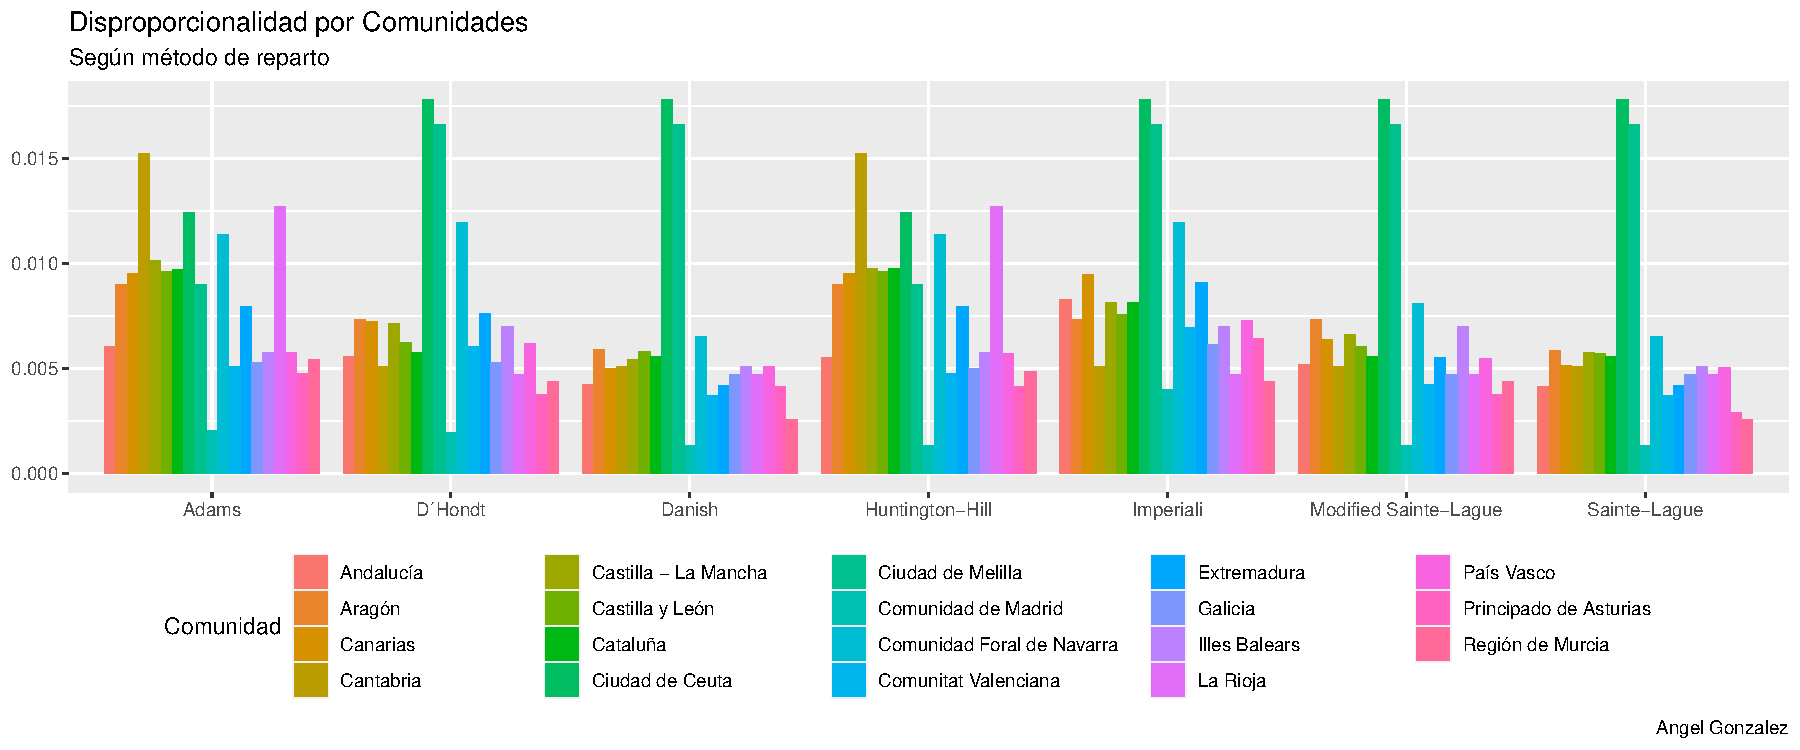
\includegraphics[width=1\linewidth]{figurasR/unnamed-chunk-30-1} \end{center}

\begin{center}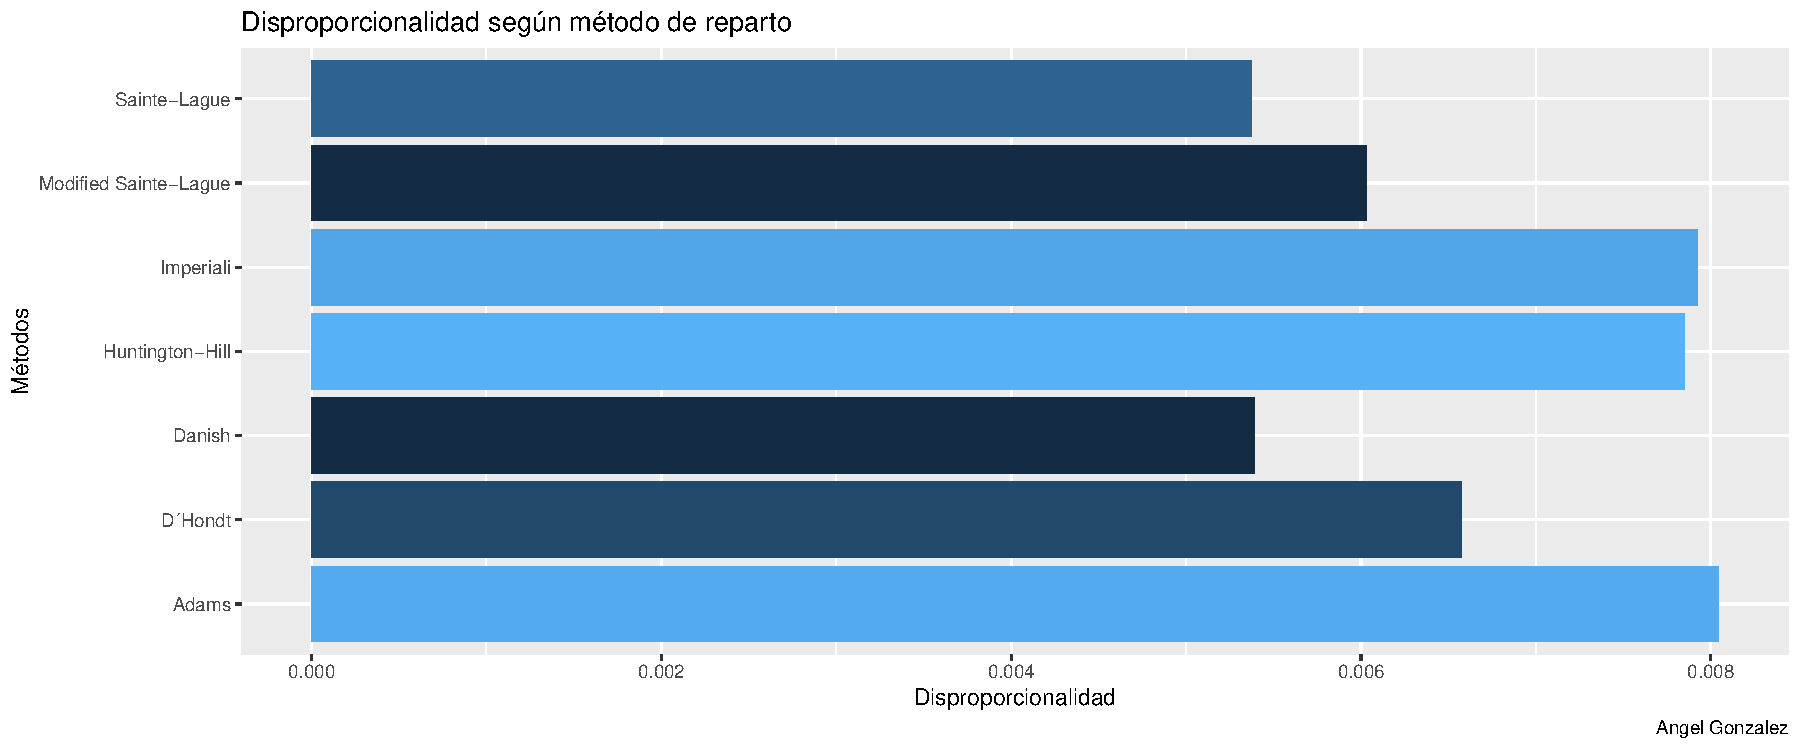
\includegraphics[width=1\linewidth]{figurasR/unnamed-chunk-30-2} \end{center}

Según el gráfico anterior por comunidades sigue la tónica general de las
anteriores elecciones, únicamente podemos apreciar en estas elecciones
una reducción de la desproporción entre comunidades, es decir, una menor
diferencia de desproporción entre ellas. Siguen dos grupos con
comportamiento similar, un grupo donde se encuentran los métodos Adams,
Huntington-Hill y LR-Imperiali, y en otro grupo los restantes. En el
caso de agrupar la desproporción por métodos observamos que el método
Imperiali vuelve a ser el más desproporcionado este año mientras que en
la parte de los métodos mas proporcionados el método mejor sería el
LR-Imperiali, LR-Hare y Sainte-Lague, el método D´Hondt utilizado en
España sigue siendo un método que se encuentra en un nivel medio, sin
destacar por una desproporción alta ni baja entre todos los métodos.

\hypertarget{auxf1o-2008}{%
\section{Año 2008}\label{auxf1o-2008}}

\hypertarget{comparativa-de-asientos-obtenidos-9}{%
\subsection{Comparativa de asientos
obtenidos}\label{comparativa-de-asientos-obtenidos-9}}

\begin{center}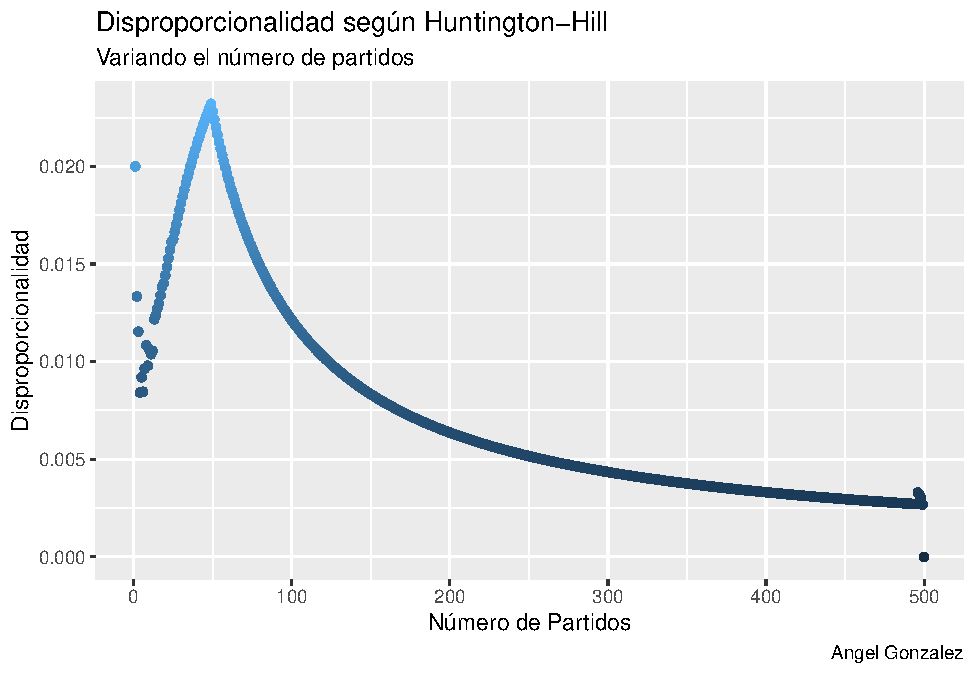
\includegraphics[width=1\linewidth]{figurasR/unnamed-chunk-32-1} \end{center}

\begin{center}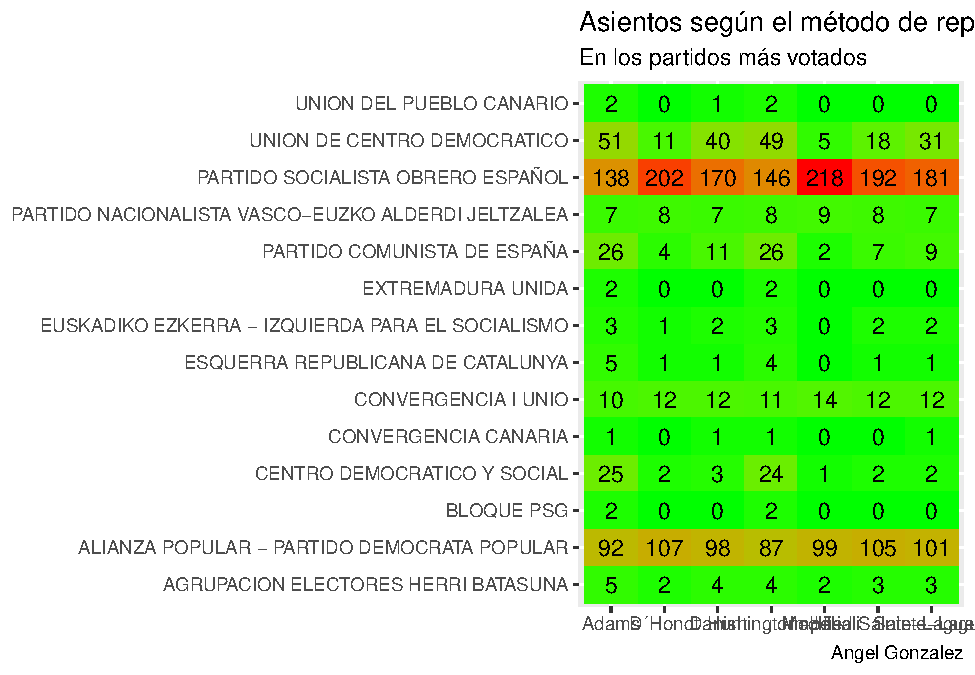
\includegraphics[width=1\linewidth]{figurasR/unnamed-chunk-32-2} \end{center}

En estos comicios del año 2008 no hay diferencias significativas en
términos de escaños, sigue un claro bipartidismo con dos partidos
hegemónicos, en primer lugar el más votado en estas elecciones que sigue
siendo el \emph{PSOE} seguido por el \emph{PP}, la diferencia de escaños
entre ellos continúa siendo prácticamente la misma pero en este año el
bipartidismo es cada vez más pronunciado, aumentando ambos partidos su
presencia en el congreso. Para el partido más votado únicamente en dos
casos podría obtener la mayoría absoluta, que sería en el caso de optar
por el método Imperiali, una mayoría absoluta justa al llegar sólo a los
175 escaños o bien por el métodos LR-Imperiali que alcanzaría los 180
escaños. Utilizando los métodos de reparto más proporcionales como son
el Danish y el Sainte-Lague la diferencia entre los partidos más votados
se reduciría a la vez que obtendrían un menor número de escaños, el
partido más perjudicado sigue siendo Izquierda Unida que podría hasta
más que quintuplicar su presencia en el congreso de haber optado por el
método Danish.

\hypertarget{desproporciuxf3n-9}{%
\subsection{Desproporción}\label{desproporciuxf3n-9}}

\begin{center}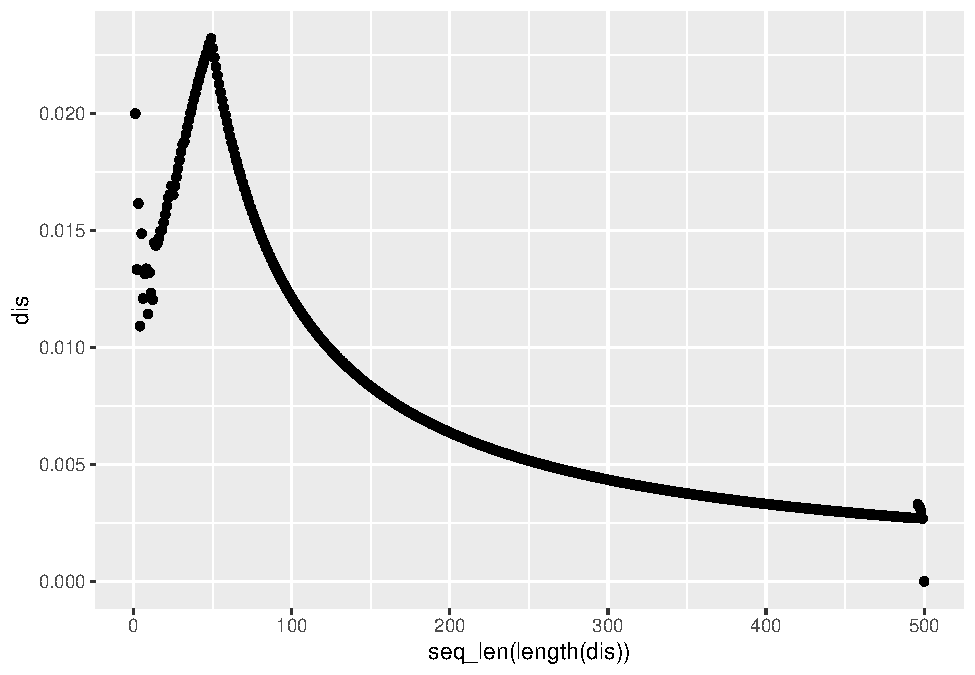
\includegraphics[width=1\linewidth]{figurasR/unnamed-chunk-33-1} \end{center}

\begin{center}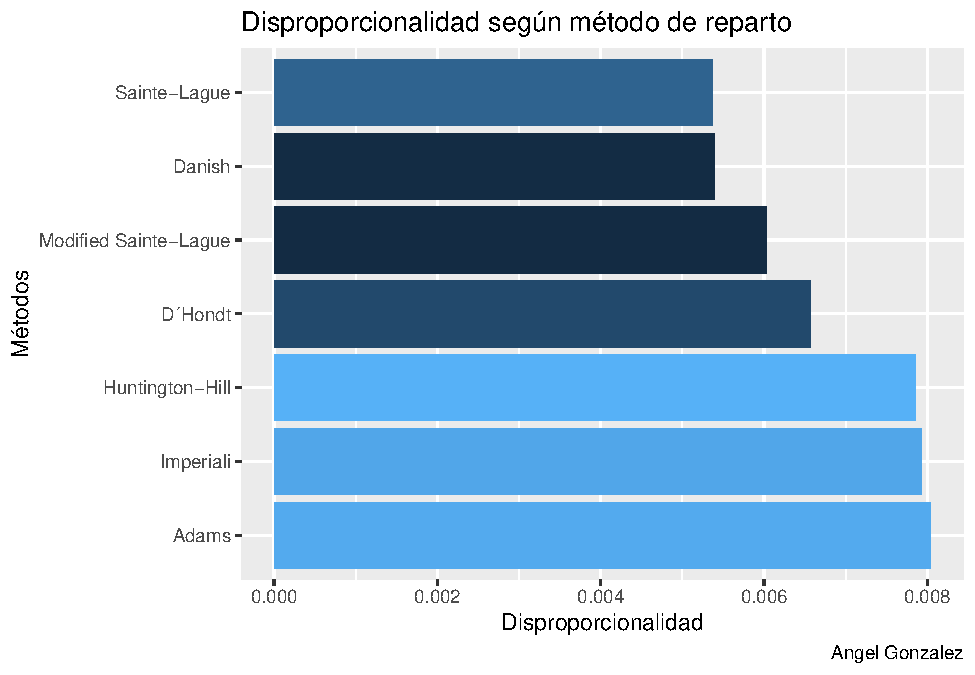
\includegraphics[width=1\linewidth]{figurasR/unnamed-chunk-33-2} \end{center}

Este es un año que se puede observar una mayor igualdad en el caso de
las desproporciones, las comunidades no tienen una gran diferencia de
proporcionalidad entre ellas sin contar con las habituales de Ceuta y
Melilla, además no encontramos grandes diferencias entre los métodos.\\
Si observamos la gráfica de la desproporción según el método de reparto
es llamativo este año que únicamente tenemos un método especialmente
despropocionado que es el Imperiali, en cambio todos los demás métodos
están en un mismo nivel con una baja diferencia entre ellos, el mejor
método en estas elecciones es el método LR-Imperiali, el método D´Hont
utilizado en España no presenta diferencias y se encuentra en un nivel
medio-alto de desproporción entre todos los métodos analizados.

\hypertarget{auxf1o-2011}{%
\section{Año 2011}\label{auxf1o-2011}}

\hypertarget{comparativa-de-asientos-obtenidos-10}{%
\subsection{Comparativa de asientos
obtenidos}\label{comparativa-de-asientos-obtenidos-10}}

\begin{center}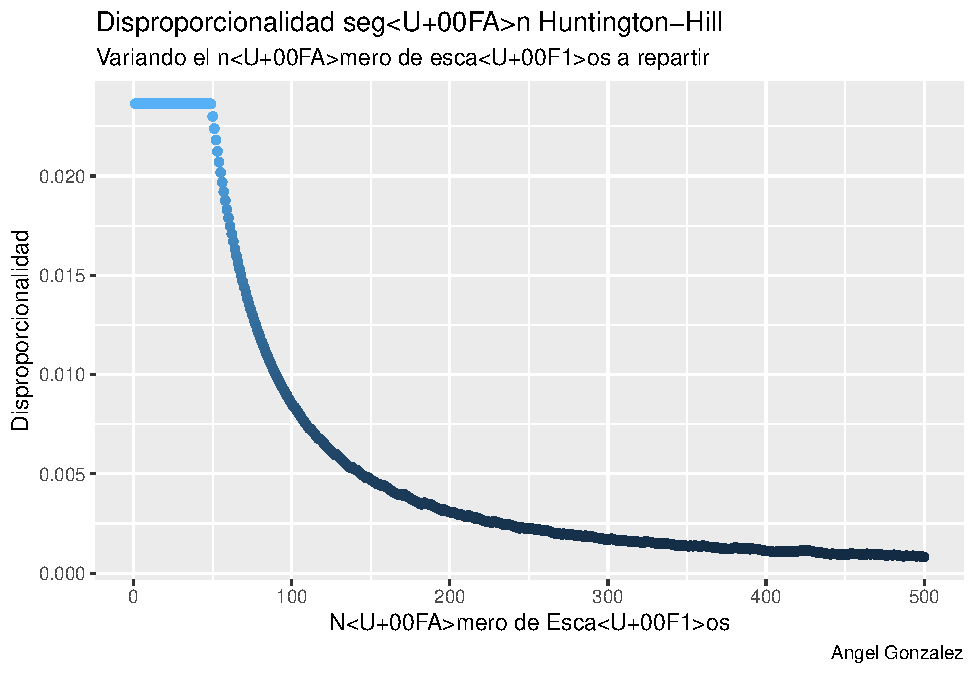
\includegraphics[width=1\linewidth]{figurasR/unnamed-chunk-35-1} \end{center}

\begin{center}\includegraphics[width=1\linewidth]{figurasR/unnamed-chunk-35-2} \end{center}

Este año 2011 podemos considerarlo como el primer año en el que aunque
continúe sucediendo un claro bipartidismo empiezan a surgir partidos
medianos con cada vez más presencia en el congreso, en este año es la
aparición de \emph{UPyD}. El partido más votado en estas elecciones es
el Partido Popular, que además obtiene la mayoría absoluta de forma
holgada según el método D´Hondt utilizado en España, le sigue el
\emph{PSOE} a una diferencia muy significativa, casi duplica la
presencia en el congreso del \emph{PP} respecto al \emph{PSOE}. Si
observamos los otros métodos propuestos vemos que el \emph{PP} en el
caso del método Danish no llegaría a obtener la mayoría absoluta pero si
utilizásemos el método de Sainte-Lague sí que alcanzaríamos la mayoría
absoluta con 176 escaños. Los partidos más perjudicados por utilizar el
método D´Hont son en estas elecciones \emph{UPyD} y \emph{IU}, los
cuales de haber optado por el método Danish podrían duplicar su
presencia en el congreso. Es llamativo el resultado de las elecciones
según el método Adams y Huntington-Hill, son métodos que dan escaños a
los partidos con menos votos en detrimento de los partidos más votados,
en estas elecciones vemos como el resultado cambiaría radicalmente, el
\emph{PP} de ser el partido más votado con mucha diferencia pasaría a
reducir la diferencia de escaños a la mitad pero la diferencia más
notoria está en los partidos medianos \emph{UPyD} y \emph{IU}, que
pasarían de 5 a 41 escaños y de 11 a 54 escaños respectivamente.

\hypertarget{desproporciuxf3n-10}{%
\subsection{Desproporción}\label{desproporciuxf3n-10}}

\begin{center}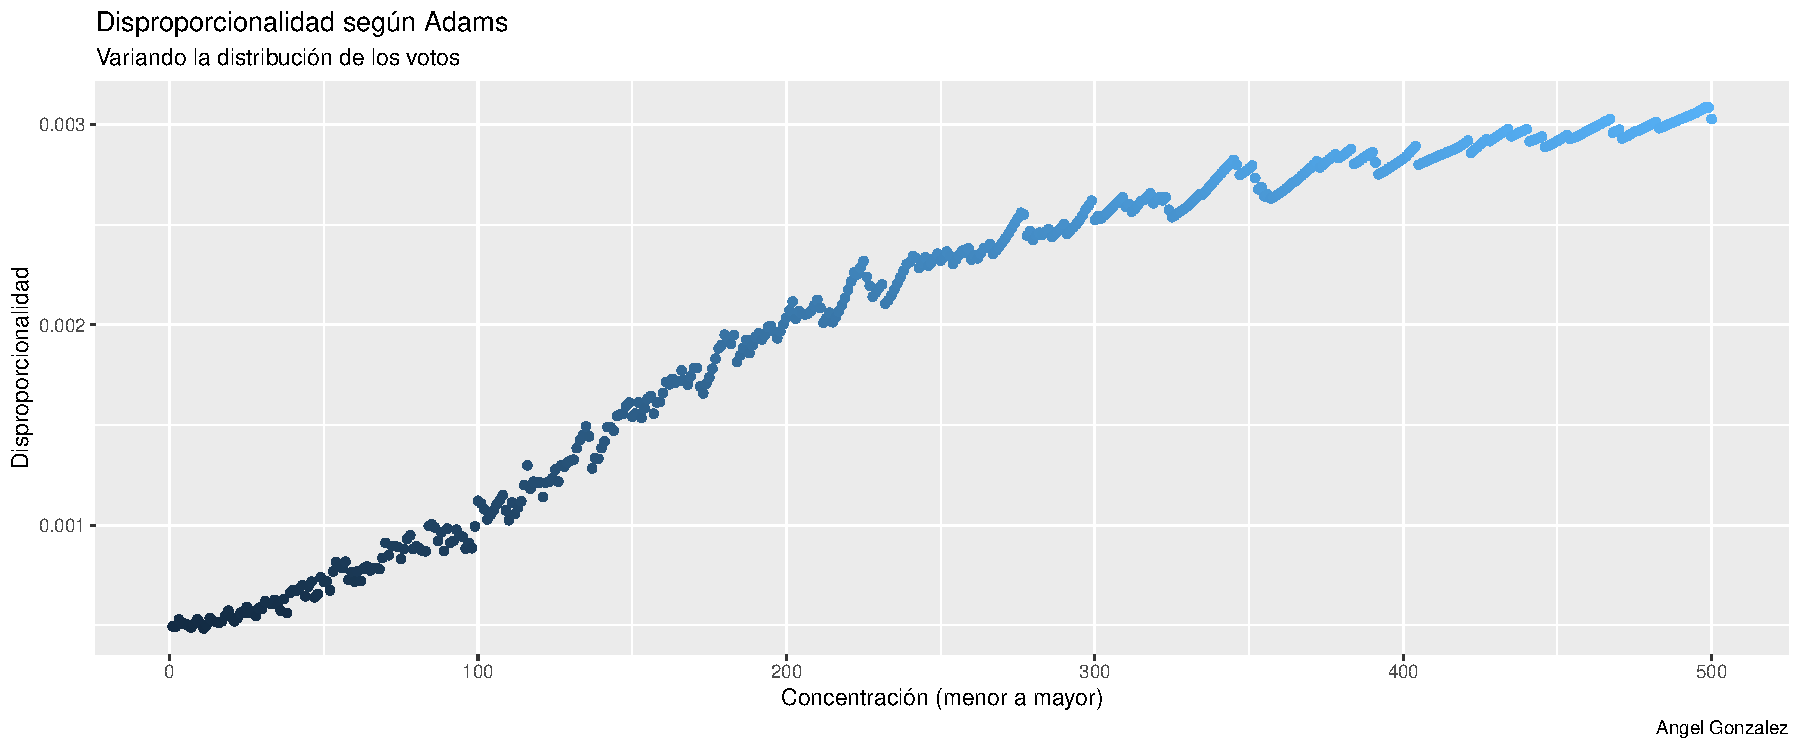
\includegraphics[width=1\linewidth]{figurasR/unnamed-chunk-36-1} \end{center}

\begin{center}\includegraphics[width=1\linewidth]{figurasR/unnamed-chunk-36-2} \end{center}

Observando el gráfico de la desproporción entre comunidades vemos como
este año particularmente el comportamiento general de todos los métodos
es similar a diferencia de las anteriores elecciones en donde los
métodos Adams y Huntington-Hill presentaban un comportamiento claramente
distinto respecto a los restantes métodos, este año el comportamiento de
todos los métodos es similar.

Si observamos la desproporción según el método de reparto volvemos a
observar dos grupos bien diferenciados, uno en el que hay una gran
desproporción, donde estarían los métodos Huntington-Hill, Adams e
Imperiali, y otro grupo con los restantes métodos con una
proporcionalidad baja. El método D´Hondt utilizado en España se
encontraría en el grupo de desproporción media, los mejores métodos en
estas elecciones son el método LR-Hare y Danish.

\hypertarget{auxf1o-2015}{%
\section{Año 2015}\label{auxf1o-2015}}

\hypertarget{comparativa-de-asientos-obtenidos-11}{%
\subsection{Comparativa de asientos
obtenidos}\label{comparativa-de-asientos-obtenidos-11}}

\begin{center}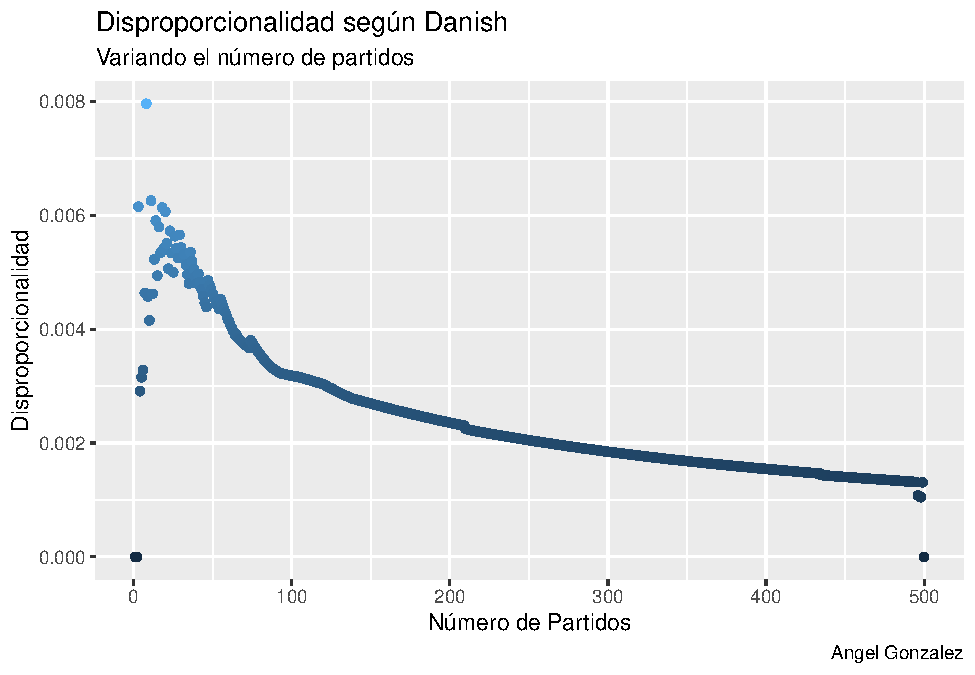
\includegraphics[width=1\linewidth]{figurasR/unnamed-chunk-38-1} \end{center}

\begin{center}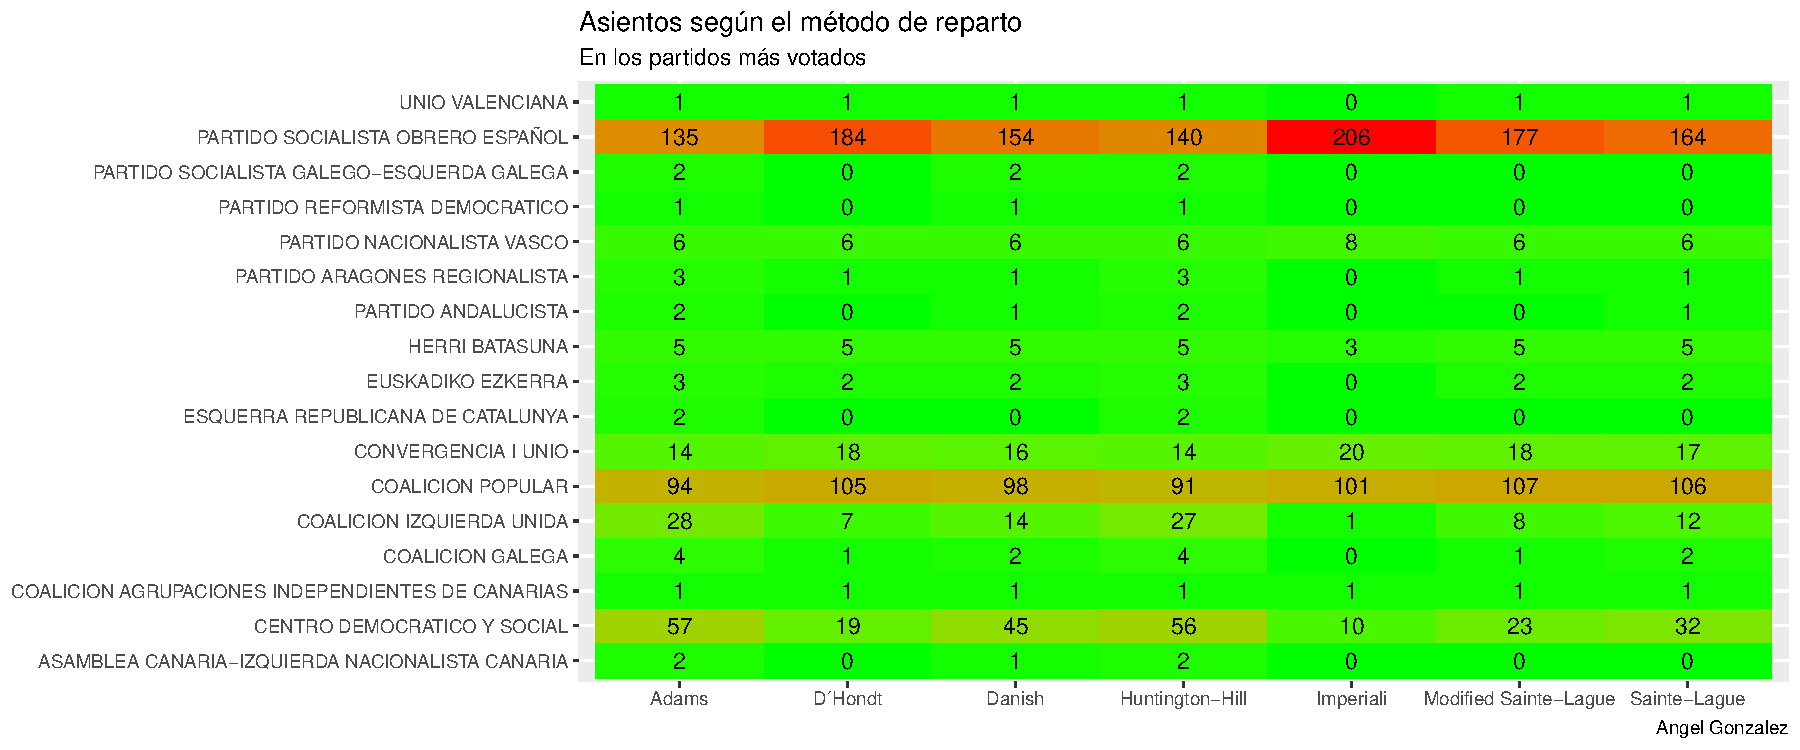
\includegraphics[width=1\linewidth]{figurasR/unnamed-chunk-38-2} \end{center}

En estas elecciones del 2014 ya vemos que el bipartidismo que veíamos
omnipresente en todas las elecciones anteriores ahora ya no ocurre, es
el primer año en el que se puede afirmar que ya no hay un bipartidismo
claro. El partido más votado es el \emph{Partido Popular} seguido por el
\emph{PSOE}, pero ya vemos que este año aparecen dos nuevos partidos
medianos, que son \emph{Podemos} y \emph{Ciudadanos.} El partido más
votado no obtiene la mayoría absoluta en ningún método, es interesante
observar como entre Podemos y Ciudadanos en el caso de utilizar el
método D´Hondt el primero superaría en dos escaños al segundo, mientras
que de haber utilizado el método Danish, Ciudadanos superaría a Podemos
en dos escaños. En el caso de optar por el método Danish, el partido más
votado, el \emph{PP}, perdería bastantes escaños y su diferencia
respecto al segundo se vería reducida significativamente. En el caso de
los partidos medianos verían su presencia en el congreso aumentar
levemente pero en ningún caso supondría un cambio significativo. El
partido más perjudicado este año vuelve a ser \emph{Izquierda Unida},
que podría pasar de obtener 2 escaños con el método D´Hondt a 11 escaños
con el Danish.

\hypertarget{desproporciuxf3n-11}{%
\subsection{Desproporción}\label{desproporciuxf3n-11}}

\begin{center}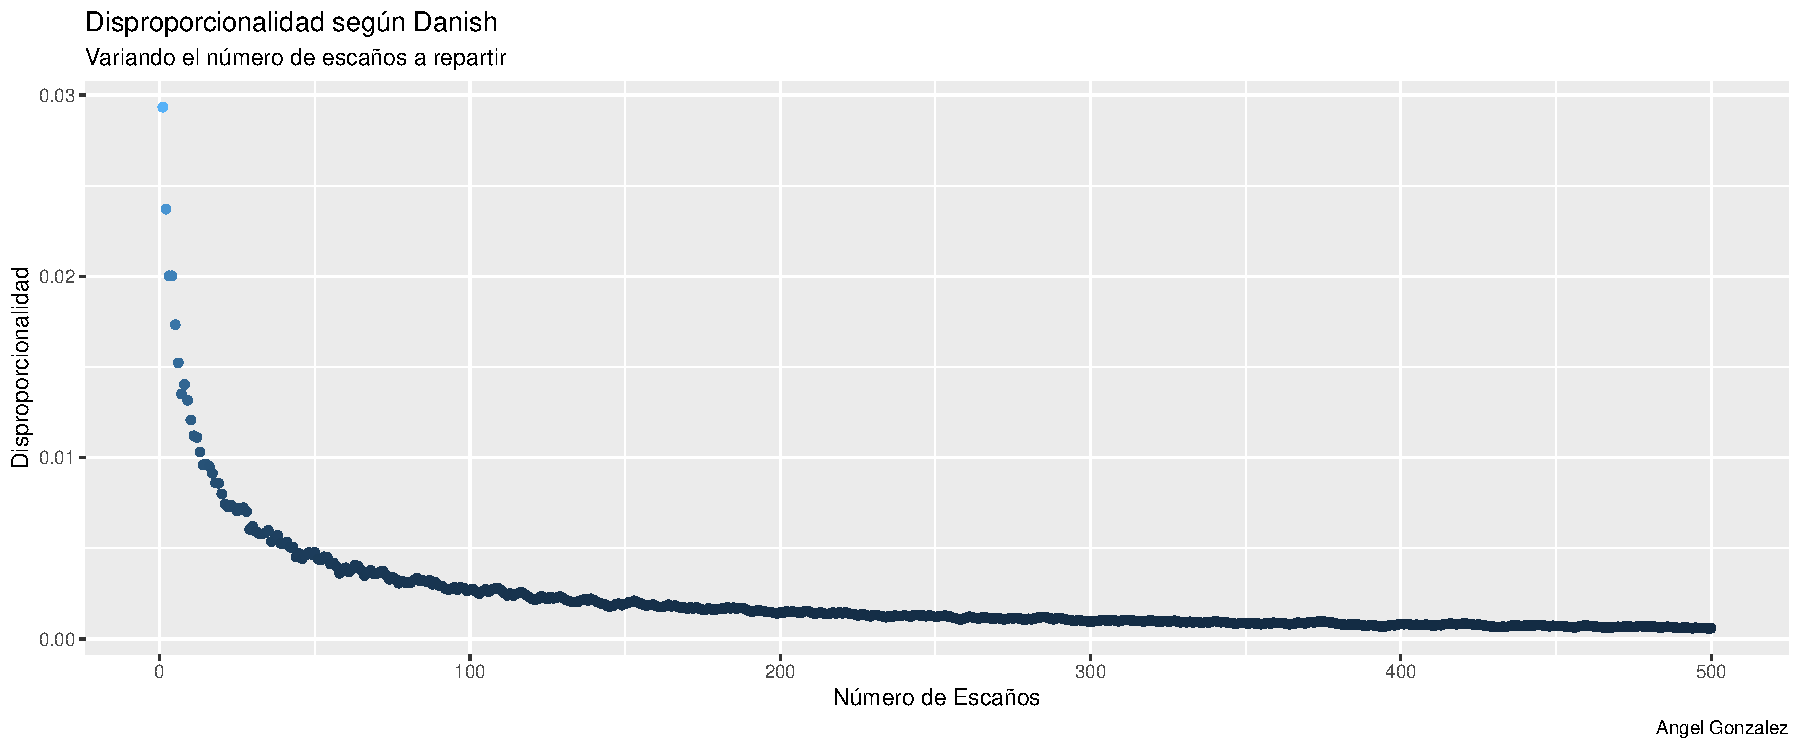
\includegraphics[width=1\linewidth]{figurasR/unnamed-chunk-39-1} \end{center}

\begin{center}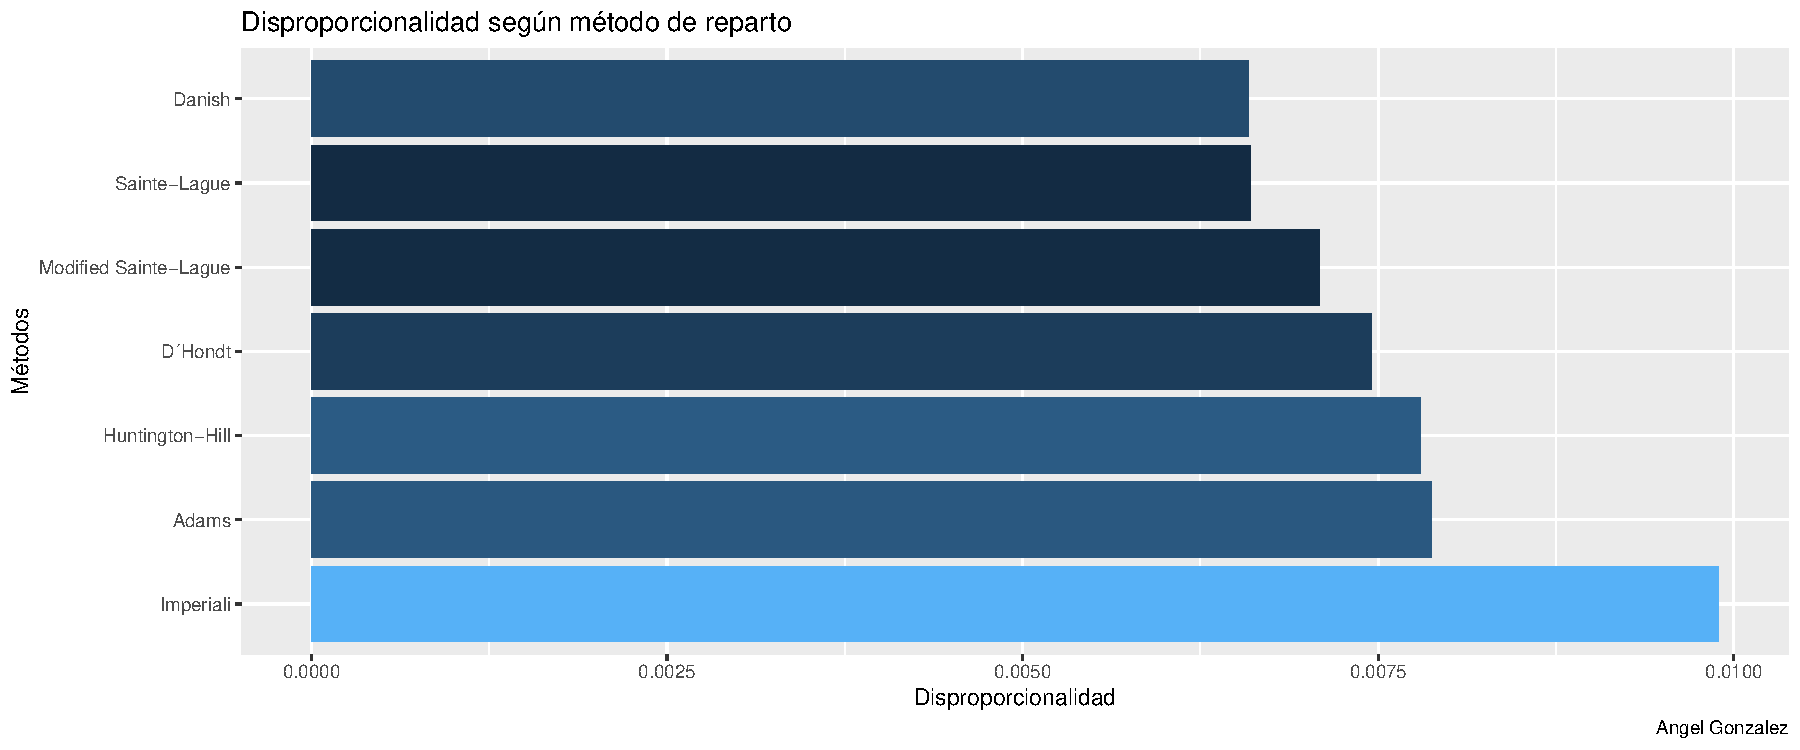
\includegraphics[width=1\linewidth]{figurasR/unnamed-chunk-39-2} \end{center}

Según el gráfico por comunidades volvemos a ver un comportamiento
claramente distinto de los demás de los métodos Adams y Huntington-Hill,
es un año en el que la diferencia de desproporción entre las distintas
comunidades aumentan. Siguen presentandose las mayores desproporciones
en Ceuta y Melilla y la menor desproporción en la comunidad de Madrid.

En el caso de la desproporción según el método de reparto este año
tenemos nuevamente dos grupos diferenciados, en un grupo con una
desproporción alta estaría el método Imperiali, LR-Droop y LR-Imperiali,
respectivamente, y todos los métodos restantes se encontrarían en el
grupo de desproporción baja, el mejor método este año es el LR-Hare y el
Sainte-Lague, encontramos que el método D´Hondt utilizado en España es
el peor método posible dentro del grupo con baja desproporción, por lo
tanto sería conveniente plantear el cambio a otro método mejor.

\hypertarget{auxf1o-2016}{%
\section{Año 2016}\label{auxf1o-2016}}

\hypertarget{comparativa-de-asientos-obtenidos-12}{%
\subsection{Comparativa de asientos
obtenidos}\label{comparativa-de-asientos-obtenidos-12}}

\begin{center}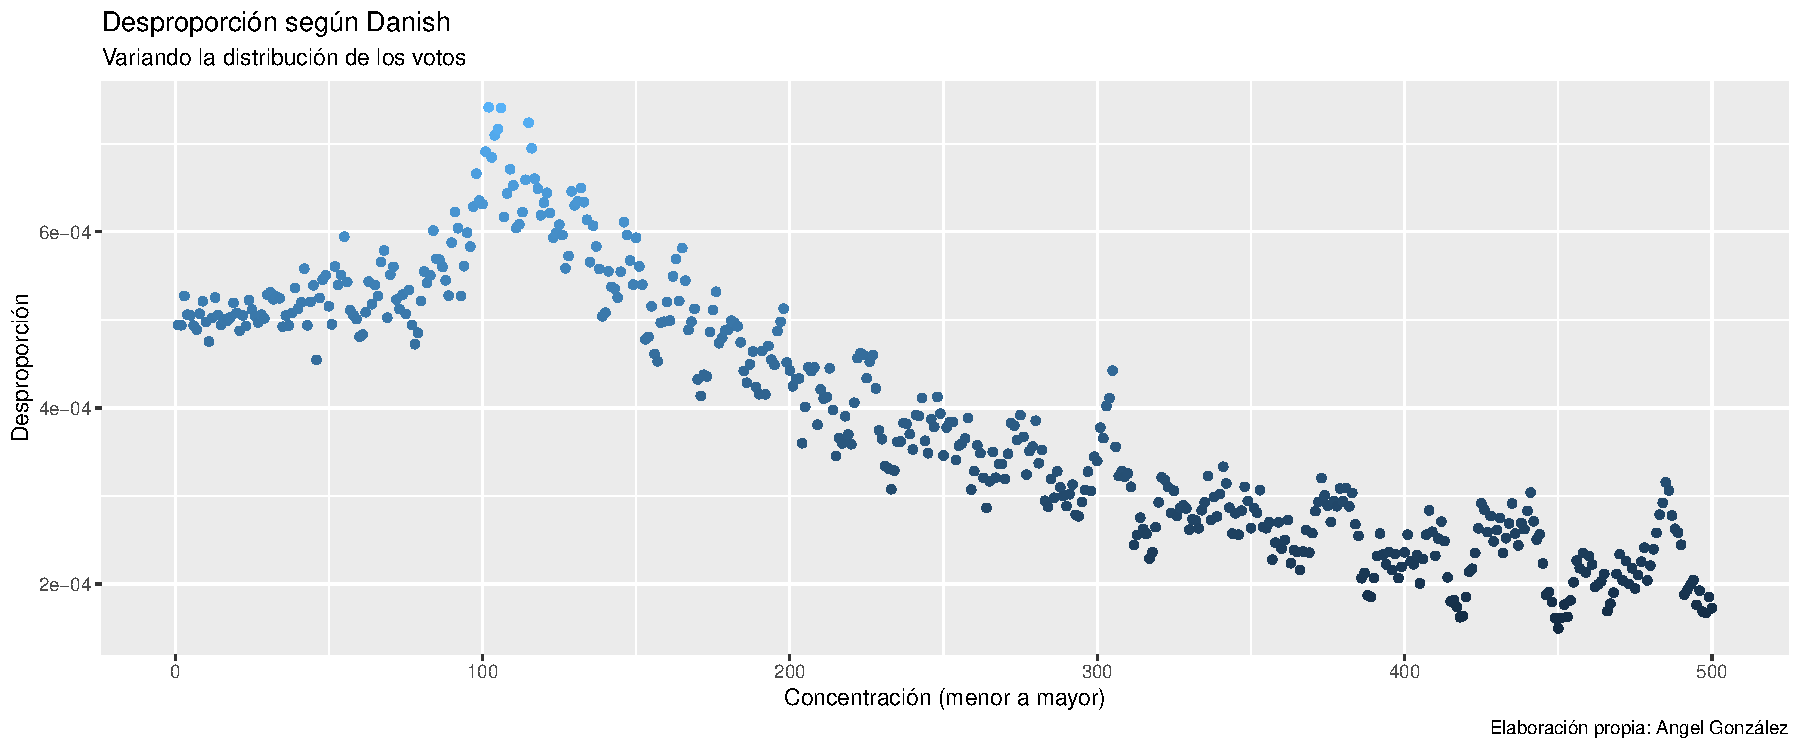
\includegraphics[width=1\linewidth]{figurasR/unnamed-chunk-41-1} \end{center}

\begin{center}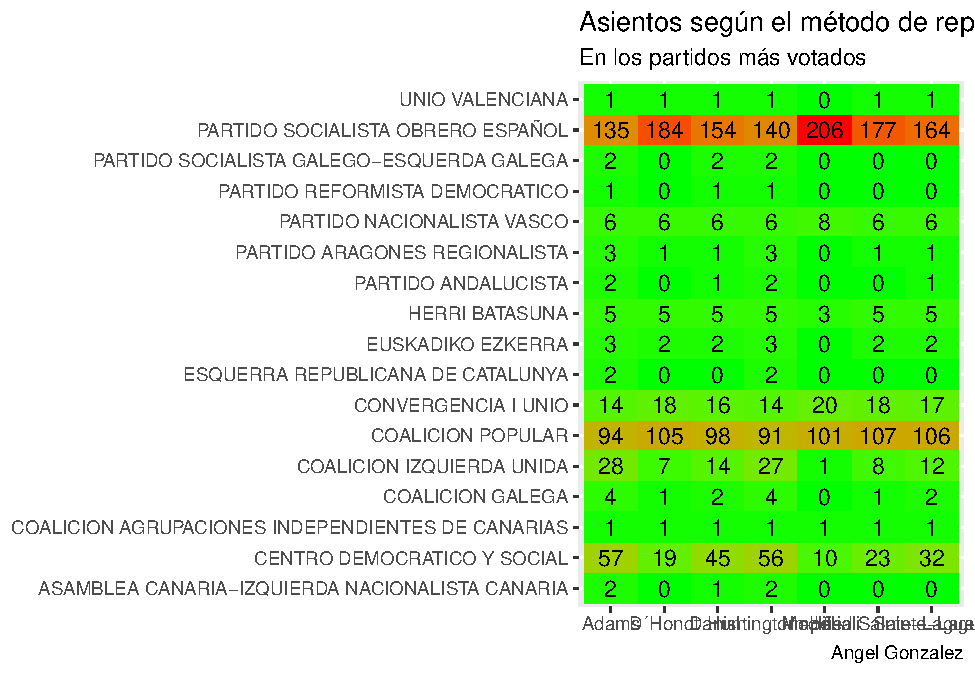
\includegraphics[width=1\linewidth]{figurasR/unnamed-chunk-41-2} \end{center}

En las elecciones del año 2016 vemos como se va consolidando el modelo
de las anteriores elecciones, con dos grandes partidos y dos partidos
medianos. La fuerza política más votada este año es el \emph{Partido
Popular} seguido del \emph{PSOE}, en ningún método el \emph{PP}
alcanzaría la mayoría absoluta, son unas elecciones que no presentan
diferencias significativas al cambiar de método de reparto, en el caso
de utilizar el método Danish respecto al D´Hondt resultaría en un menor
número de escaños para el \emph{PP} y una ligera subida de escaños de
\emph{Podemos} y \emph{Ciudadanos.} Son las primeras elecciones en donde
el método de reparto no cambia significativamente el reparto de escaños,
es notorio que en este año el \emph{PSOE} obtenga casi los mismos votos
independientemente del método utilizado.

\hypertarget{desproporciuxf3n-12}{%
\subsection{Desproporción}\label{desproporciuxf3n-12}}

\begin{center}\includegraphics[width=1\linewidth]{figurasR/unnamed-chunk-42-1} \end{center}

\begin{center}\includegraphics[width=1\linewidth]{figurasR/unnamed-chunk-42-2} \end{center}

En la desproporción por comunidades vemos el habitual comportamiento
entre los métodos, con el método Adams y el Huntington-Hill
comportándose diferente a los demás. Respecto a las diferencias de
desproporción entre comunidades este año es especialmente similar el
comportamiento aunque con distinta magnitud entre los distintos métodos.
En el gráfico en que comparamos los métodos de reparto el comportamiento
es similar al anterior año, con un método que es significativamente
desproporcionado respecto a los demás, el método Imperiali, y los demás
métodos muy similares entre ellos siendo el mejor el método LR-Hare y
Sainte-Lague, el método utilizado en España, el D´Hondt, vuelve a ser de
los peores por lo que cada vez sería más necesario proponer un cambio de
método de reparto a otro más proporcional.

\hypertarget{auxf1o-2019-abril}{%
\section{Año 2019, Abril}\label{auxf1o-2019-abril}}

\hypertarget{comparativa-de-asientos-obtenidos-13}{%
\subsection{Comparativa de asientos
obtenidos}\label{comparativa-de-asientos-obtenidos-13}}

\begin{center}\includegraphics[width=1\linewidth]{figurasR/unnamed-chunk-44-1} \end{center}

\begin{center}\includegraphics[width=1\linewidth]{figurasR/unnamed-chunk-44-2} \end{center}

En estas elecciones de Abril de 2019 vemos como ya no existe el
bipartidismo, este año podemos agrupar a los partidos políticos en
cuatro categorías, la primera en donde hay un partido con muchos votos
con una gran diferencia de escaños respecto a los demás, que es el
\emph{PSOE}, un segundo grupo en donde se encontrarían dos partidos con
un número medio-alto de escaños, que son el \emph{PP} y
\emph{Ciudadanos} respectivamente, un tercer grupo con un número mediano
de escaños con \emph{Podemos} y \emph{Vox}, y un último grupo de pocos
escaños con los demás partidos. Este año tampoco hay una diferencia
significativa de haber utilizado un método de reparto respecto a otro,
los partidos más perjudicados por la elección del método D´Hondt son
\emph{Vox} y \emph{Podemos}, en ningún caso el partido más votado
alcanza la mayoría absoluta. De haber utilizado el método Danish el
partido que se vería más beneficiado sería \emph{Vox} seguido de
\emph{Ciudadanos}, partido que superaría en escaños al \emph{PP} y se
convertiría en la segunda fuerza en el hemiciclo.

\hypertarget{desproporciuxf3n-13}{%
\subsection{Desproporción}\label{desproporciuxf3n-13}}

\begin{center}\includegraphics[width=1\linewidth]{figurasR/unnamed-chunk-45-1} \end{center}

\begin{center}\includegraphics[width=1\linewidth]{figurasR/unnamed-chunk-45-2} \end{center}

Este es un año en el que viendo la desproporción por comunidades es
especialmente similar independientemente del método utilizado, siguen
presentándose dos grupos de distinto comportamiento, dentro de los dos
grupos todos los métodos siguen un patrón de desproporción similar, sin
olvidar el comportamiento habitual de las ciudades de Ceuta y Melilla y
de la comunidad de Madrid como la provincia más proporcionada.

Cuando comparamos la proporcionalidad según el método de reparto sucede
algo que no se había visto hasta ahora, que un método que anteriormente
a llegado a ser el más desproporcionado sucede que este año es el más
proporcionado, este método es el Huntington-Hill, en el extremo opuesto
está el método Imperiali con una diferencia bastante significativa
respecto a las demás. El método utilizado en España vuelve a ser uno de
los peores, en estas elecciones el cuarto peor, parece ser un método que
no está preparado para ser óptimo en escenarios en donde no hay un
bipartidismo claro.

\hypertarget{auxf1o-2019-noviembre}{%
\section{Año 2019, Noviembre}\label{auxf1o-2019-noviembre}}

\hypertarget{comparativa-de-asientos-obtenidos-14}{%
\subsection{Comparativa de asientos
obtenidos}\label{comparativa-de-asientos-obtenidos-14}}

\begin{center}\includegraphics[width=1\linewidth]{figurasR/unnamed-chunk-47-1} \end{center}

\begin{center}\includegraphics[width=1\linewidth]{figurasR/unnamed-chunk-47-2} \end{center}

En esta gráfica de las elecciones de Noviembre de 2019 podemos observar
una ligera recuperación del bipartidismo en donde los dos principales
partidos vuelven a aumentar el número de escaños obtenidos y también
aumentar la diferencia en escaños respecto a los demás. Son unas
elecciones en donde hay dos partidos principales, que son el \emph{PSOE}
y el \emph{PP} respectivamente, uno medio en escaños, \emph{Vox}, y tres
partidos de un nivel medio-bajo de escaños, que son \emph{Podemos},
\emph{ERC} y \emph{Ciudadanos} respectivamente. En el caso de optar por
otro método en ninguno de ellos se alcanzaría la mayoría absoluta. Hay
dos partidos perjudicados por utilizar el método D´Hondt en vez de otro
más proporcional como pueda ser el Danish, son los partidos de
\emph{Podemos} que pasarían de obtener 26 escaños a 40 y el partido
\emph{Ciudadanos} que pasaría a duplicar su presencia de 10 escaños a
23.

\hypertarget{desproporciuxf3n-14}{%
\subsection{Desproporción}\label{desproporciuxf3n-14}}

\begin{center}\includegraphics[width=1\linewidth]{figurasR/unnamed-chunk-48-1} \end{center}

\begin{center}\includegraphics[width=1\linewidth]{figurasR/unnamed-chunk-48-2} \end{center}

En el gráfico por comunidades obtenemos el mismo comportamiento que en
las elecciones anteriores sin obtener una diferencia significativa.
Cuando comparamos la desproporción según el método de reparto el método
de Imperiali sigue siendo el más desproporcionado mientras que el mejor
método esta vez resulta ser el LR-Hare y Sainte-Lague, el método D´Hondt
como hemos visto en anteriores elecciones sigue siendo el cuarto peor
método posible entre todos los analizados.

\hypertarget{comparativa-entre-auxf1os}{%
\section{Comparativa entre años}\label{comparativa-entre-auxf1os}}

En este apartado final procederemos a agrupar todos los resultados de la
desproporción, los agruparemos por año y método. Con todo ello
realizaremos dos gráficos, uno en el que muestre la desproporción a lo
largo de los años distinguiendo el método de reparto utilizado y otro en
el que muestre el promedio de la desproporción a lo largo de todos los
años analizados para cada método.

\begin{center}\includegraphics[width=1\linewidth]{figurasR/unnamed-chunk-49-1} \end{center}

\begin{center}\includegraphics[width=1\linewidth]{figurasR/unnamed-chunk-49-2} \end{center}

En este gráfico comparando la desproporción media por año observamos
como la desproporción desde las elecciones de 1977 hasta 1989 está en un
nivel medio, a partir del año 1993 la desproporción baja, principalmente
debido a un bipartidismo más marcado, esto se mantiene hasta el año de
las elecciones de 2011, en donde empieza por primera vez a aparecer un
tercer partido que debilita el bipartidismo por lo que la desproporción
aumenta a los niveles de las primeras elecciones de 1977, desde el año
2011 hasta las últimas elecciones de 2019 la desproporción se mantiene
sin mucha variación.

En el gráfico de la desproporción según el método de reparto podemos
extraer conclusiones para decidir cual método ha sido el mejor a lo
largo de todas las elecciones realizadas en España a partir de 1977, por
lo tanto sacamos estas conclusiones:

\begin{itemize}
\tightlist
\item
  El mejor método es el Saint-Lague por parte de los métodos de promedio
  mayor y por los métodos de resto mayor el mejor método es el LR-Hare.
\item
  El peor método entre todos los analizados es con diferencia el método
  Imperiali.
\item
  El método utilizado en España, el método D´Hondt, es el sexto mejor
  método en términos de proporcionalidad.
\end{itemize}

Por lo tanto al preguntarnos si el método utilizado en España es el
mejor método en términos de desproporción que se puede utilizar para el
reparto de los escaños podemos afirmar que no lo es, de hecho se sitúa
en la mitad de la tabla entre todos los métodos analizados, la
característica que tiene el método D´Hont es que se sitúa entre los
métodos que benefician más a los partidos más votados y de entre ellos
es el método más proporcional, por lo que se podría decir que es el
método más proporcional entre los métodos que ``facilitan la
gobernanza''. Si nuestro objetivo es obtener la máxima proporcionalidad
en vez de facilitar la gobernanza deberíamos plantear un cambio de
método, en primer lugar al Sainte-Lague o al Danish en el caso de los
métodos de promedio mayor, ambos métodos son casi idénticos en términos
de proporcionalidad pero el Sainte-Lague tiene una mejor característica
que el Danish, que reparte los escaños de forma que es más fácil
gobernar, o bien al método LR-Hare en el caso de los métodos de resto
mayor. En cambio si queremos facilitar la gobernanza a la vez que
tratamos de minimizar la desproporción entre los escaños y los votos, en
este caso el método D´Hondt es donde muestra su valor, puesto que es
como hemos comentado anteriormente, el método que entra dentro del grupo
que benefician más a los partidos más votados y de entre ellos es el
método más proporcional, por esta razón se puede considerar el método
más equilibrado para el gobierno de una nación.

\bibliography{bib/library.bib,bib/paquetes.bib}


\addcontentsline{toc}{chapter}{Bibliografía}


\end{document}
